% concatenated from FDBGK_0907_.tex
\documentclass[10pt,reqno]{amsart}

\usepackage[margin=1in]{geometry}
\usepackage{amsmath,amssymb,amsthm,mathtools}
\usepackage{mathrsfs}
\usepackage{enumitem}
\usepackage{microtype}
\usepackage{graphicx}
\usepackage{float}
\usepackage{tikz}
\usetikzlibrary{arrows.meta,positioning}
\numberwithin{equation}{section}

\usepackage[dvipsnames]{xcolor}
\usepackage[colorlinks=true,linkcolor=blue,urlcolor=blue,citecolor=PineGreen]{hyperref}
% \usepackage{refcheck}
\usepackage{sidecap}
\usepackage[normalem]{ulem}

\newtheorem{theorem}{Theorem}[section]
\newtheorem{proposition}{Proposition}[section]
\newtheorem{lemma}{Lemma}[section]
\newtheorem{corollary}{Corollary}[section]
\newtheorem{remark}{Remark}[section]
\theoremstyle{definition}
\newtheorem{definition}{Definition}[section]

\newcommand{\R}{\mathbb R}
\newcommand{\dd}{\mathrm d}
\newcommand{\dx}{\mathrm{d}x}
\newcommand{\dpp}{\mathrm{d}p}
\newcommand{\dt}{\mathrm{d}t}
\newcommand{\ds}{\mathrm{d}s}
\newcommand{\dy}{\mathrm{d}y}
\newcommand{\dr}{\mathrm{d}r}
\newcommand{\dtheta}{\mathrm{d}\theta}
\newcommand{\be}{B^{\varepsilon}}
\newcommand{\kappah}{\kappa_{\hbar}}
\newcommand{\e}{\varepsilon}
\newcommand{\one}{\mathbf 1}


%MathCal Characters
\newcommand{\calA}{\mathcal A}
\newcommand{\calB}{\mathcal B}
\newcommand{\calC}{\mathcal C}
\newcommand{\calD}{\mathcal D}
\newcommand{\calE}{\mathcal E}
\newcommand{\calF}{\mathcal F}
\newcommand{\calG}{\mathcal G}
\newcommand{\calH}{\mathcal H}
\newcommand{\calI}{\mathcal I}
\newcommand{\calJ}{\mathcal J}
\newcommand{\calK}{\mathcal K}
\newcommand{\calL}{\mathcal L}
\newcommand{\calM}{\mathcal M}
\newcommand{\calN}{\mathcal N}
\newcommand{\calO}{\mathcal O}
\newcommand{\calP}{\mathcal P}
\newcommand{\calQ}{\mathcal Q}
\newcommand{\calR}{\mathcal R}
\newcommand{\calS}{\mathcal S}
\newcommand{\calT}{\mathcal T}
\newcommand{\calU}{\mathcal U}
\newcommand{\calV}{\mathcal V}
\newcommand{\calW}{\mathcal W}
\newcommand{\calX}{\mathcal X}
\newcommand{\calY}{\mathcal Y}
\newcommand{\calZ}{\mathcal Z}

\newcommand{\bq}{\begin{equation}}
\newcommand{\eq}{\end{equation}}
\newcommand{\lt}{\left}
\newcommand{\rt}{\right}
\newcommand{\pa}{\partial}


%   SS  
\usepackage[colorinlistoftodos]{todonotes}

\newcommand{\boxsihyun}[1]{\todo[inline,color=MidnightBlue!20]{{\bf Sihyun:} #1}}

\usepackage{cancel}

%%%%%%%%%%%%%%%%%%%%%%%%


\title{Global mild solutions and the semiclassical limit for the Fermi--Dirac BGK model}

\author[Choi]{Young-Pil Choi}
\address[Young-Pil Choi]{\newline Department of Mathematics\newline
Yonsei University, 50 Yonsei-Ro, Seodaemun-Gu, Seoul 03722, Republic of Korea}
\email{ypchoi@yonsei.ac.kr}

\author[Hwang]{Byung-Hoon Hwang}
\address[Byung-Hoon Hwang]{\newline Department of Mathematics Education\newline
	Sangmyung University, 20 Hongjimun 2-gil, Jongno-Gu, Seoul 03016, Republic of Korea}
\email{bhhwang@smu.ac.kr}

 \author[Song]{Sihyun Song}
 \address[Sihyun Song]{\newline Department of Mathematics\newline
 Yonsei University, 50 Yonsei-Ro, Seodaemun-Gu, Seoul 03722, Republic of Korea}
 \email{ssong@yonsei.ac.kr}

\begin{document}

\allowdisplaybreaks

 

\date{\today}

 \keywords{Quantum BGK model, Fermi--Dirac statistics, global mild solutions, Pauli exclusion principle, saturation, semiclassical limit.}

\begin{abstract}
We prove global existence of mild solutions to the spatially inhomogeneous Fermi--Dirac BGK equation for arbitrary-size Pauli-admissible initial data with finite mass and kinetic energy, allowing both vacuum and locally saturated zero-temperature states. The construction relies on a moment-compatible regularization of the local equilibrium that preserves the Pauli bound and uniform moment control while remaining consistent up to the saturation boundary. The solutions satisfy mass, momentum, and energy conservation and, under an additional finite spatial second-moment assumption, an entropy-gap H-theorem on the full Pauli interval.  Under uniform moment and entropy bounds, we further prove that, after extraction of a subsequence, quantum mild solutions converge strongly in phase space, uniformly on bounded time intervals, to a mild solution of the classical BGK equation.
\end{abstract}

\maketitle \centerline{\date}


 

 



\tableofcontents
 

%%%%%%%%%%%%%%%%%%%%%%%%%%%%%%%%%%%%%%%%%%%%%%%
%
%
%
%
%
%
%%%%%%%%%%%%%%%%%%%%%%%%%%%%%%%%%%%%%%%%%%%%%%%
\section{Introduction}
%%%%%%%%%%%%%%%%%%%%%%%%%%%%%%%%%%%%%%%%%%%%%%%
%
%
%
%
%
%
%%%%%%%%%%%%%%%%%%%%%%%%%%%%%%%%%%%%%%%%%%%%%%%
\subsection{The Fermi--Dirac BGK equation}

In this paper we study the Fermi--Dirac BGK equation
\bq \label{eq:FD-BGK}
\pa_t f+p\cdot\nabla_x f=\calF(f)-f,  \quad  (t,x,p)\in(0,\infty)\times\R^3\times\R^3,
\eq
where $\hbar>0$ is the quantum parameter and the Pauli exclusion principle is represented by
\[
 0\leq f\leq\frac1\hbar .
\]
Here $\calF(f)$ denotes the Fermi--Dirac local equilibrium associated with the quantum parameter $\hbar$. The collision operator in \eqref{eq:FD-BGK} is a relaxation-time approximation of the fermionic quantum Boltzmann equation associated with Fermi--Dirac statistics \cite{UU33}.

For a nonnegative distribution $f$, set
\[
 N_f(t,x):=\int_{\R^3}f(t,x,p)\,\dpp,  \quad  P_f(t,x):=\int_{\R^3}pf(t,x,p)\,\dpp,  \quad  E_f(t,x):=\int_{\R^3}|p|^2f(t,x,p)\,\dpp.
\]
The case $N_f(t,x)=0$ is immediate: nonnegativity implies $f(t,x,\cdot)=0$ almost everywhere, and we set $\calF(f)(t,x,\cdot)=0$.  Thus, we describe the local equilibrium on the non-vacuum set $\{N_f>0\}$.

Define
\[
 u_f:=\frac{P_f}{N_f},  \quad  \calE_f:=E_f-\frac{|P_f|^2}{N_f}.
\]
The quantity $\calE_f$ is the kinetic energy relative to the local mean velocity $u_f$, since
\[
 \calE_f  =  \int_{\R^3}|p-u_f|^2f(t,x,p)\,\dpp. 
 \]  
As will be shown below, the Pauli constraint implies the sharp inequality
\bq \label{eq:pa-b}
 \calE_f\geq \kappah N_f^{\frac53},  \quad  \kappah:=  \frac{3^{\frac53}}{5(4\pi)^{\frac23}}\hbar^{\frac23}.
\eq
Accordingly, the local equilibrium appearing in \eqref{eq:FD-BGK} is given by
\bq \label{eq:F-s}
 \calF(f)(t,x,p)
 =
 \begin{cases}
 \displaystyle  \frac{1}{  \exp \lt(  a_f(t,x)|p-u_f(t,x)|^2+c_f(t,x)  \rt)+\hbar},  &  \calE_f(t,x) >\kappah N_f(t,x)^{\frac53},  \\[3mm]
 \displaystyle  \frac1\hbar  \one_{\{|p-u_f(t,x)|\leq R_f(t,x)\}},  &  \calE_f(t,x) = \kappah N_f(t,x)^{\frac53},
 \end{cases}
\eq
where
\[
 R_f:=\lt(\frac{3\hbar N_f}{4\pi}\rt)^{\frac13}.
\]
The first line of \eqref{eq:F-s} is the finite-temperature Fermi--Dirac equilibrium, whereas the second line is its saturated zero-temperature endpoint.  We next describe how the parameters $a_f$ and $c_f$ in the first case are determined by the macroscopic moments and why the threshold in \eqref{eq:pa-b} is the natural one.

For $N>0$, set
\[
 B(N,P,E):=  \frac{N}{(E-|P|^2/N)^{\frac35}},  \quad  B_f:=B(N_f,P_f,E_f).
\]
For $k\geq0$, define
\[
 \beta_k^{\hbar}(c):=  \int_{\R^3}  \frac{|p|^k}{e^{|p|^2+c}+\hbar}\,\dpp,  \quad  \beta^{\hbar}(c):=  \frac{\beta_0^{\hbar}(c)}{\beta_2^{\hbar}(c)^{\frac35}}.
\]
The particular combination defining $B$ and $\beta^{\hbar}$ follows directly from the scaling of the Fermi--Dirac family.  Indeed, for
\[
 F_{a,c,u}(p):=  \frac1{e^{a|p-u|^2+c}+\hbar},  \quad a>0,
\]
the change of variables $q=\sqrt a\,(p-u)$ gives
\[
 N_{F_{a,c,u}} =a^{-\frac32}\beta_0^{\hbar}(c), \quad P_{F_{a,c,u}} =uN_{F_{a,c,u}},\quad  E_{F_{a,c,u}}  -\frac{|P_{F_{a,c,u}}|^2}{N_{F_{a,c,u}}} =a^{-\frac52}\beta_2^{\hbar}(c).
\]
Eliminating $a$ from these identities yields
\[
 B(  N_{F_{a,c,u}},  P_{F_{a,c,u}},  E_{F_{a,c,u}})  =  \beta^{\hbar}(c).
\]
Thus $B$ is the macroscopic quantity invariant under the temperature scaling of the family, while $\beta^{\hbar}$ is the corresponding equilibrium moment map.

The function $\beta^{\hbar}$ is strictly decreasing from $\R$ onto $(0,\beta^{\hbar}(-\infty))$, where
\[
 \beta^{\hbar}(-\infty)  =  \frac{5^{\frac35}(4\pi)^{\frac25}}  {3\hbar^{\frac25}}.
\]
See Lemma \ref{lem:beta} below.  Hence, whenever
\[
 0<B_f<\beta^{\hbar}(-\infty),
\]
there exists a unique $c_f\in\R$ satisfying
\[
 \beta^{\hbar}(c_f)=B_f,  \quad  a_f:=  \beta_0^{\hbar}(c_f)^{\frac23}N_f^{-\frac23}.
\]
The coefficient $a_f$ is the nondimensional inverse-temperature scale, whereas $c_f$ is a chemical-potential-type parameter.

The relation between the range of $B$ and the two cases in \eqref{eq:F-s} follows from the sharp Pauli inequality.  Lemma \ref{lem:sharp-pauli} shows that
\[
 \calE_f\geq\kappah N_f^{\frac53},  \quad  \kappah=\beta^{\hbar}(-\infty)^{-\frac53}.
\]
Consequently,
\[
 \calE_f>\kappah N_f^{\frac53}  \quad\Longleftrightarrow\quad  B_f<\beta^{\hbar}(-\infty),
\]
which is precisely the finite-temperature regime in the first line of \eqref{eq:F-s}.  At the endpoint,
\[
 \calE_f=\kappah N_f^{\frac53}  \quad\Longleftrightarrow\quad  B_f=\beta^{\hbar}(-\infty),
\]
the unique admissible distribution with the prescribed moments
is
\[
 \frac1\hbar  \one_{\{|p-u_f|\leq R_f\}},
\]
which gives the second line of \eqref{eq:F-s}.

The latter distribution is the zero-temperature endpoint of the finite-temperature Fermi--Dirac family.  Indeed, writing
\[
 a_f|p-u_f|^2+c_f  =  a_f\lt(|p-u_f|^2-\mu_f\rt),  \quad  \mu_f:=-\frac{c_f}{a_f},
\]
one sees that, as the inverse-temperature scale becomes large, the transition across the level $|p-u_f|^2=\mu_f$ becomes sharp.  We refer to the resulting profile as the saturated zero-temperature Fermi--Dirac distribution; the sphere $|p-u_f|=R_f$ is the Fermi surface in the present isotropic setting.

An intrinsic formulation, useful also at the endpoint, is provided by the Fermi--Dirac entropy.  Define
\[
 \eta_\hbar(z)  :=  z\log z  +\frac1\hbar(1-\hbar z)\log(1-\hbar z),  \quad  0\leq z\leq\frac1\hbar ,
\]
with the convention $0\log0=0$. Proposition \ref{prop:vari} shows that, for every non-vacuum moment triple $(N,P,E)$ arising from a Pauli-admissible distribution, the equilibrium $\calF[N,P,E]$ is the unique minimizer of
\[
 \int_{\R^3}\eta_\hbar(g)\,\dpp
\]
under the Pauli constraint and the prescribed mass, momentum, and energy.  Related quantum entropy optimization problems are discussed in \cite{EMV05}.  In particular, both regimes in \eqref{eq:F-s} satisfy the moment identities
\[
 \int_{\R^3}(1,p,|p|^2)  \lt(\calF(f)-f\rt) \dpp=0.
\]

For the classical BGK equation, global existence and stability based on compactness of the macroscopic fields, velocity-moment estimates, and entropy were established in \cite{Per89}. Weighted $L^\infty$ estimates and uniqueness were subsequently obtained in \cite{PP93}. Smooth solutions near a global Maxwellian and their large-time behavior were later studied in \cite{Yun10}. For the ES--BGK model, global theories are available both near equilibrium and, for fixed collision frequency, for large initial data \cite{HY19,Yun15JDE,Yun15SIAM}; multicomponent models and large-amplitude stability have also been developed in \cite{BKPY23,BKLY26}.

For the fermionic BGK model itself, the available time-dependent Cauchy theory is primarily perturbative. A global classical theory near a Fermi--Dirac equilibrium is given in \cite{BY20}, while stationary mild solutions in a slab are constructed in \cite{BY20S} under conditions that rule out a transition to a saturated local state. Related quantum BGK models include stationary and multi-species variants. Nouri \cite{Nou08} proved existence of bounded measure solutions for a stationary Bose--Einstein BGK model in a slab, while a multi-species BGK model associated with the Uehling--Uhlenbeck equation, including the well-definedness of its implicitly determined equilibrium parameters and its conservation and entropy structures, was developed in \cite{BKPY21}. Related quantum relaxation models have been treated in analytic or perturbative regimes \cite{Bra19,Bra20}, and global near-equilibrium theories are available for quantum Boltzmann equations \cite{BJY21,OW22}.

The zero-temperature branch is, however, a familiar feature of fermionic kinetic theory beyond BGK.  For the spatially homogeneous Boltzmann--Fermi--Dirac equation, the equilibrium classification contains both finite-temperature Fermi--Dirac distributions and saturated characteristic functions of momentum balls \cite{Lu01}; stability and strong convergence for this dynamics are studied in \cite{LW03}, and recent hard-potential results further develop the homogeneous theory and explicitly distinguish the saturated equilibrium case \cite{AP25p}.  Saturated equilibria and the degeneracy associated with the Pauli upper bound also play an important role for the Landau--Fermi--Dirac equation \cite{ABDL22,BL04,GGZ22}.  Spatially inhomogeneous weak-solution theories for the Boltzmann--Fermi--Dirac equation are available in the whole-space, general-domain, and periodic settings \cite{All10,Dol94,Lu08}; for harder interactions, global classical solutions near equilibrium have also been obtained \cite{JZ25}. More recently, global weak solutions and semiclassical analysis have been developed for the spatially inhomogeneous Coulomb Landau--Fermi--Dirac equation \cite{Sam24p,Sam26}.  These results show that saturation is a genuine and well-established feature of fermionic kinetic equations.  For the spatially inhomogeneous Fermi--Dirac BGK equation, however, incorporating this endpoint into a global large-data mild theory requires control of the nonlinear local equilibrium throughout the full Pauli-admissible moment region.

A separate line of work concerns semiclassical limits of fermionic kinetic equations.  For the spatially homogeneous quantum Boltzmann equation, the vanishing-quantum-parameter limit has been justified first at the level of weak convergence and subsequently through quantitative asymptotic expansions; see \cite{HLP21,HLPZ24}.  In the spatially inhomogeneous setting, the semiclassical limit from the Coulomb Landau--Fermi--Dirac equation to a renormalized solution of the classical Landau equation has recently been established in \cite{Sam26}.  These results concern collision operators whose semiclassical analysis is tied to the specific Boltzmann or Landau structure.  For the Fermi--Dirac BGK equation considered here, the quantum dependence is instead concentrated in an implicitly determined local equilibrium.  To the best of our knowledge, a rigorous semiclassical limit from the spatially inhomogeneous Fermi--Dirac BGK equation to the classical BGK equation has not previously been established.

%%%%%%%%%%%%%%%%%%%%%%%%%%%%%%%%%%%%%%%%%%%%%%%
%
%
%
%
%
%
%%%%%%%%%%%%%%%%%%%%%%%%%%%%%%%%%%%%%%%%%%%%%%%

\subsection{Main results}

Our first result treats arbitrary-size Pauli-admissible initial data with finite mass and kinetic energy for the spatially inhomogeneous Fermi--Dirac BGK equation in $\R_x^3$.  We construct global mild solutions that allow vacuum and permit the local moments to reach the sharp Pauli boundary corresponding to a saturated zero-temperature equilibrium. To the best of our knowledge, this is the first global large-data existence result for this equation covering the full range of Pauli-admissible local moments.

This goes beyond the available perturbative Cauchy theory, where the solution remains close to a fixed finite-temperature equilibrium, and the stationary slab theory, where the assumptions exclude a transition to a saturated local state.  In the present setting, vacuum and saturated local states are both admitted in the solution class.  Consequently, neither a positive lower bound on the local density nor a uniform separation from the Pauli boundary is available.
 
The main difficulty is to control the nonlinear local equilibrium simultaneously near vacuum and near saturation. The bulk velocity $P_f/N_f$ becomes singular as the density vanishes, whereas the finite-temperature parametrization degenerates as the moment triple approaches the sharp Pauli boundary. We first characterize the admissible moment region by the sharp Pauli inequality and define the equilibrium variationally on this entire region, including its saturated boundary.

A key methodological ingredient is a moment-compatible regularization of this equilibrium map. The issue is not merely to smooth the macroscopic parameters: the approximation must simultaneously remain Pauli-admissible, become Lipschitz for each fixed regularization parameter, and retain moment bounds that are uniform as the regularization is removed. We achieve this by coupling the regularization of the density and bulk velocity with a range truncation of the degeneracy parameter and a compatible interpolation near vacuum. At non-vacuum points, the resulting profiles remain within the finite-temperature Fermi--Dirac family, and the regularized equilibrium satisfies
\[
 \int_{\R^3}(1+|p|^2)\calF^\e(f)(p)\,\dpp \leq C_\hbar(N_f+E_f),
\]
with $C_\hbar$ independent of $\e$. In particular, the approximation does not introduce an additive energy background near vacuum. The fixed-$\e$ Lipschitz bound and this uniform moment estimate serve distinct purposes: the former yields the regularized solutions, while the latter permits the compactness argument. The regularization is also consistent for converging moment triples whose limits lie on the saturation boundary; see Lemmas \ref{lem:unif-e} and \ref{lem:fix-e-Lip} and Proposition \ref{prop:consist}.

Identification of the collision term requires strong compactness of the local energy in addition to the density and momentum. Spatial tightness, velocity averaging, and a local third-moment estimate based on the geometry of free trajectories in $\R_x^3$ provide the required compactness. The continuity of the moment-to-equilibrium map then identifies the nonlinear relaxation term, even at saturated limit points.

Exact conservation and entropy dissipation are recovered at the level of the limiting equation, rather than imposed on the regularized dynamics. The approximation preserves the Pauli bound and the uniform moment estimates, and its mass defect tends to zero. After passage to the limit, exact local moment matching yields mass, momentum, and energy conservation directly from the mild formulation. The entropy inequality requires a further argument since $\eta_\hbar'$ has logarithmic singularities at both endpoints of the Pauli interval. Hence, we use the entropy-gap dissipation and approximate $\eta_\hbar'$ by bounded monotone functions, preserving convexity of the entropy approximation. This yields the H-theorem on the full Pauli interval, including saturated zero-temperature states.


For functions on phase space, we use
\[
 \|g\|_{L^1_2}  :=  \iint_{\R^3\times\R^3}  (1+|p|^2)|g(x,p)|\,\dx\dpp,
\]
and, for functions of momentum alone,
\[
 \|g\|_{L^1_2(\R^3_p)}  :=  \int_{\R^3}(1+|p|^2)|g(p)|\,\dpp.
\]
We also define
\bq \label{eq:H-def}
 \mathscr H_\hbar(g)  :=  \iint_{\R^3\times\R^3}  \eta_\hbar(g)\,\dx\dpp
\eq
and
\bq \label{eq:D-def}
 \mathscr D_\hbar(g)  :=  \int_{\R^3}  \lt(  \int_{\R^3}\eta_\hbar(g)\,\dpp  -  \int_{\R^3}\eta_\hbar(\calF(g))\,\dpp  \rt)\dx.
\eq
By the variational characterization of the local equilibrium, $\mathscr D_\hbar(g)\geq0$ (see Proposition \ref{prop:vari}).

With this notation, our first main theorem gives the global construction of a mild solution together with the conservation laws and the entropy inequality.

\begin{theorem}\label{thm:main}
Assume
\bq \label{eq:ini}
 0\leq f_0\leq\frac1\hbar \quad\text{a.e.},  \quad  \|f_0\|_{L^1_2}<\infty.
\eq
Then there exists
\[
 f\in C([0,\infty);L^1(\R^3\times\R^3)) \cap L^\infty([0,\infty);L^1_2(\R^3\times\R^3))
\]
such that $0\leq f\leq\frac1\hbar $ almost everywhere and
\bq \label{eq:mild-main}
 f(t,x,p) =e^{-t}f_0(x-tp,p) +\int_0^t e^{-(t-s)} \calF(f)(s,x-(t-s)p,p)\,\ds
\eq
for every $t\geq0$ in $L^1(\R^3\times\R^3)$.  Moreover,
\[
 \iint_{\R^3\times\R^3}  (1,p,|p|^2)f(t,x,p)\,\dx\dpp  =  \iint_{\R^3\times\R^3}  (1,p,|p|^2)f_0(x,p)\,\dx\dpp
\]
for every $t\geq0$.

If, in addition,
\[
 \iint_{\R^3\times\R^3}  |x|^2f_0(x,p)\,\dx\dpp<\infty,
\]
then $\mathscr H_\hbar(f(t))$ is finite for every $t\geq0$, $\mathscr D_\hbar(f)\in L^1_{\rm loc}([0,\infty))$, and
\bq\label{eq:H-thm-gap}
 \mathscr H_\hbar(f(t))  +  \int_0^t\mathscr D_\hbar(f(s))\,\ds  \leq  \mathscr H_\hbar(f_0)  \quad\text{for every }t\geq0.
\eq
\end{theorem}

\begin{remark}
The entropy-gap formulation is convenient since it remains finite and well defined on the entire Pauli interval, including the endpoint values $f=0$ and $f=\frac1\hbar $.  On the finite-temperature region, a stronger logarithmic entropy production can be recovered under additional integrability assumptions excluding the endpoint singularities.  Indeed, writing $F=\calF(f)$, define formally
\[
 \mathscr D_\hbar^{\log}(f)  :=  \iint_{\R^3 \times \R^3}  (f-F)  \lt(  \log\frac{f}{1-\hbar f}  -  \log\frac{F}{1-\hbar F}  \rt) \dx\dpp .
\]
Equivalently,
\[
 \mathscr D_\hbar^{\log}(f) = \iint_{\R^3 \times \R^3}  (f-F)  \log\lt(  \frac{f(1-\hbar F)}{F(1-\hbar f)}  \rt) \dx\dpp
 \ge0.
\]
When $F$ is a finite-temperature equilibrium, we get $\eta_\hbar'(F)  =  -a|p-u|^2-c$, and exact local moment matching gives
\[
 \int_{\R^3} \eta_\hbar'(F)(f-F)\,\dpp=0.
\]
Thus, whenever the logarithmic terms are integrable, the characteristic chain rule yields the stronger entropy identity
\[
\mathscr H_\hbar(f(t))  +  \int_0^t\mathscr D_\hbar^{\log}(f(s))\,\ds  =  \mathscr H_\hbar(f_0).
\]
Moreover, by convexity,
\[
 \mathscr D_\hbar^{\log}(f)\ge  \mathscr D_\hbar(f).
\]
If $f$ reaches $0$ or $\frac1\hbar $, however, the logarithmic production may fail to be finite, whereas the entropy-gap dissipation $\mathscr D_\hbar$ remains meaningful.  At a saturated point, the sharp Pauli inequality (Lemma \ref{lem:sharp-pauli} below) forces $f=\calF(f)$ almost everywhere in momentum, hence the entropy gap vanishes automatically.
\end{remark}
 

\begin{remark}
Strict separation from the Pauli ceiling is propagated for all positive times.  More precisely, assume in addition that
\[
 f_0(x,p)<\frac1\hbar   \quad\text{for almost every }(x,p).
\]
Then the mild formula and $0\le\calF(f)\le\frac1\hbar $ give, for every $t>0$,
\[
 f(t,x,p) \le  e^{-t}f_0(x-tp,p)  +  \frac1\hbar \int_0^t e^{-(t-s)}\,ds   =  e^{-t}f_0(x-tp,p)  +(1-e^{-t})\frac1\hbar   <\frac1\hbar 
\]
for almost every $(x,p)$.  Hence equality in the sharp Pauli inequality (Lemma \ref{lem:sharp-pauli} below) is impossible at almost every non-vacuum point. This means
\[
 E_f(t,x)-\frac{|P_f(t,x)|^2}{N_f(t,x)}  >  \kappa_\hbar N_f(t,x)^{\frac53}
\]
almost everywhere on $\{N_f>0\}$.  Consequently, the local equilibrium $\calF(f)$ remains on the finite-temperature Fermi--Dirac branch for all positive times.

Similarly, if $f_0>0$ almost everywhere, then
\[
 f(t,x,p)\ge e^{-t}f_0(x-tp,p)>0.
\]
 Lemma \ref{lem:sharp-pauli} tells us that this also excludes the possibility of the local equilibrium $\calF(f)$ being saturated. 
\end{remark}


Theorem \ref{thm:main} concerns the quantum equation for a fixed $\hbar>0$.  Our second main result addresses the complementary question of whether the corresponding quantum solutions recover the classical BGK dynamics in the semiclassical regime $\hbar\to0$.  To state the result, for a nonnegative classical distribution $g$ with $N_g>0$, define
\[
 u_g:=\frac{P_g}{N_g},  \quad  T_g:=\frac{E_g-|P_g|^2/N_g}{3N_g},
\]
and the local Maxwellian
\[
 M(g)(t,x,p)  :=  \frac{N_g}{(2\pi T_g)^{\frac32}}  \exp \lt(-\frac{|p-u_g|^2}{2T_g}\rt).
\]
At every non-vacuum point, $T_g>0$, since an $L^1(\R^3_p)$ distribution with positive mass cannot be supported at a single velocity. At points where $N_g=0$, we set $M(g)=0$.

The compactness mechanism required for the semiclassical limit is different from the fixed-$\hbar$ construction.  For each fixed $\hbar>0$, the Pauli bound supplies the $L^2$ control used in the proof of Theorem \ref{thm:main}, whereas this control degenerates as $\hbar\to0$.  The uniform entropy bound instead gives equiintegrability. We combine bounded renormalizations with $L^1$ velocity averaging and then remove the renormalization by a quantitative $L\log L$ estimate. Together with the local third-moment bound, this yields strong compactness of the density, momentum, and energy. A second issue is the identification of the $\hbar$-dependent local equilibria.  Their parameters are determined implicitly by the Fermi--Dirac moment map, while the saturation threshold itself varies with $\hbar$.  At every non-vacuum limit point, positivity of the classical internal energy places the quantum equilibria eventually in the finite-temperature branch as $\hbar\to0$.  Compactness of the equilibrium parameters, together with local uniform convergence of the Fermi--Dirac moment map to its classical counterpart, then identifies the limiting equilibrium with the Maxwellian.  This gives strong convergence of the collision terms and ultimately the $C([0,T];L^1(\R^3\times\R^3))$ convergence in Theorem \ref{thm:semi}.

The following theorem shows that, under uniform moment and entropy bounds, every sequence of the quantum mild solutions constructed above admits a subsequence converging strongly to a mild solution of the classical BGK equation.

\begin{theorem}\label{thm:semi}
Let $\hbar_n\downarrow0$, and assume
\bq \label{eq:semi-ini-conv}
 0\leq f_{0,n}\leq\hbar_n^{-1},  \quad  f_{0,n}\to f_0  \quad\text{strongly in }L^1(\R^3\times\R^3),
\eq
for some $f_0\geq0$.  Suppose also that
\bq \label{eq:semi-ini-b}
 \sup_n  \iint_{\R^3\times\R^3}  (1+|x|^2+|p|^2)f_{0,n}\,\dx\dpp<\infty,  \quad  \sup_n  \iint_{\R^3\times\R^3}  f_{0,n}|\log f_{0,n}|\,\dx\dpp<\infty.
\eq
Let $f_n$ be global mild solutions supplied by Theorem \ref{thm:main} with $\hbar=\hbar_n$ and initial data $f_{0,n}$.  Then, after extraction of a subsequence,
\bq \label{eq:semi-f-str}
 f_n\to f  \quad\text{strongly in }  C([0,T];L^1(\R^3\times\R^3))  \quad\text{for every }T>0,
\eq
where $f$ satisfies
\[
\pa_t f+p\cdot\nabla_xf=M(f)-f,  \quad  f|_{t=0}=f_0,
\]
in the mild sense, namely
\bq \label{eq:classical-mild}
 f(t,x,p) =e^{-t}f_0(x-tp,p) +\int_0^t e^{-(t-s)}  M(f)(s,x-(t-s)p,p)\,\ds.
\eq
\end{theorem}

The assumptions on the approximating initial data in Theorem \ref{thm:semi} are satisfied by the canonical Pauli truncation of any classical datum with finite moments and entropy.  Thus every such datum admits an approximating quantum family covered by Theorem \ref{thm:semi}.

\begin{corollary}\label{cor:canon}
Assume $f_0\geq0$, and
\[
 \iint_{\R^3\times\R^3}  (1+|x|^2+|p|^2)f_0\,\dx\dpp<\infty,  \quad  \iint_{\R^3\times\R^3}  f_0|\log f_0|\,\dx\dpp<\infty.
\]
For $0<\hbar\leq1$, set
\[
 f_0^\hbar:=\min\lt\{f_0,\frac1\hbar\rt\}.
\]
Then, for every sequence $\hbar_n\downarrow0$, the initial data $f_{0,n}:=f_0^{\hbar_n}$ satisfy the assumptions of Theorem \ref{thm:semi}.  Consequently, the corresponding quantum mild solutions possess a subsequence converging strongly in $C([0,T];L^1(\R^3\times\R^3))$ for every $T>0$ to a mild solution of the classical BGK equation with initial datum $f_0$.
\end{corollary}


\begin{remark} 
Theorem \ref{thm:semi} also clarifies what happens to the zero-temperature branch in the semiclassical regime.  For fixed $\hbar>0$, the Pauli constraint imposes the sharp lower bound
\[
 E-\frac{|P|^2}{N}  \geq  \kappah N^{\frac53},  \quad  \kappah  =  \frac{3^{\frac53}}{5(4\pi)^{\frac23}}\hbar^{\frac23},
\]
and equality corresponds to the saturated Fermi--Dirac equilibrium.  As $\hbar\to0$,
\[
 \kappah\to0,  \quad  \beta^{\hbar}(-\infty)  =  \frac{5^{\frac35}(4\pi)^{\frac25}}  {3\hbar^{\frac25}}  \to\infty.
\]
Thus, at every non-vacuum point of the $L^1$ limit, where the internal energy is necessarily positive, the quantum equilibria eventually belong to the finite-temperature branch.  This explains why the limiting equilibrium in Theorem \ref{thm:semi} is a Maxwellian rather than a saturated profile.

The saturated branch does, however, have a different formal semiclassical limit.  For fixed mass $N>0$ and velocity $u$, the saturated equilibrium is
\[
 F_\hbar^{\rm sat}(p)  =  \frac1\hbar  \one_{\{|p-u|\leq R_\hbar\}},  \quad  R_\hbar  =  \lt(\frac{3\hbar N}{4\pi}\rt)^{\frac13}.
\]
As $\hbar\to0$, its support shrinks to $p=u$ while its height diverges, and
\[
 F_\hbar^{\rm sat}  \rightharpoonup N\delta_u
\]
in the sense of measures.  Hence following the zero-temperature boundary leads to a monokinetic measure rather than an $L^1$ Maxwellian.  This concentration regime is excluded by the assumptions of Theorem \ref{thm:semi}; in particular,
\[
 \int_{\R^3}  F_\hbar^{\rm sat}  |\log F_\hbar^{\rm sat}|\,\dpp  =  N|\log\hbar|  \to \infty.
\]
Thus the semiclassical limit considered here describes the positive-temperature classical BGK regime, while the simultaneous zero-temperature and semiclassical limit would constitute a different, measure-valued limiting problem.
\end{remark}
 

The rest of the paper is organized as follows. In Section \ref{sec:approx}, we discuss the moment structure of Fermi--Dirac equilibria, construct the regularized collision operator, and establish the corresponding regularized solutions. In Section \ref{sec:pass-eps}, we obtain compactness of the macroscopic moments and identify the limiting collision term, thereby completing the construction in Theorem \ref{thm:main}.  Section \ref{sec:H-thm} establishes the conservation laws and the entropy inequality.  Finally, Section \ref{sec:semiclas} proves the semiclassical limit stated in Theorem \ref{thm:semi} and verifies the canonical Pauli approximation in Corollary \ref{cor:canon}.

%%%%%%%%%%%%%%%%%%%%%%%%%%%%%%%%%%%%%%%%%%%%%%%
%
%
%
%
%
%
%%%%%%%%%%%%%%%%%%%%%%%%%%%%%%%%%%%%%%%%%%%%%%%
\section{Regularization of the Fermi--Dirac equilibrium}\label{sec:approx}

In this section we construct the regularized collision operator used in the proof of Theorem \ref{thm:main} and establish the estimates required for the limit $\e\to0$.  We first describe the admissible moment region, then introduce the regularized macroscopic parameters and the exact equilibrium map, and finally solve the regularized equation. 

Since Theorem \ref{thm:main} is concerned with the existence theory for fixed $\hbar>0$, throughout this section we omit the dependence on $\hbar$ whenever there is no risk of confusion.

%%%%%%%%%%%%%%%%%%%%%%%%%%%%%%%%%%%%%%%%%%%%%%%
%
%
%
%
%
%
%%%%%%%%%%%%%%%%%%%%%%%%%%%%%%%%%%%%%%%%%%%%%%%

\subsection{Moment identities and the admissible region}

We begin with the general Fermi--Dirac profile
\[
 F(p):=\frac{1}{e^{a|p-b|^2+c}+\hbar},  \quad a>0,\quad b\in\R^3,\quad c\in\R,
\]
and we recall
\[
 \beta_0(c)=\int_{\R^3}\frac{1}{e^{|p|^2+c}+\hbar}\,\dpp,  \quad  \beta_2(c)=\int_{\R^3}\frac{|p|^2}{e^{|p|^2+c}+\hbar}\,\dpp.
\]
A direct change of variables gives
\bq \label{eq:FD-mom-com}
 N_F=a^{-\frac32}\beta_0(c),\quad  P_F=bN_F,\quad  E_F=a^{-\frac52}\beta_2(c)+|b|^2N_F.
\eq
Thus, if $a=\beta_0(c)^{\frac23}N^{-\frac23}$, then
\bq\label{eq:FD-mom}
 N_F=N,\quad  E_F=\beta(c)^{-\frac53}N^{\frac53}+N|b|^2.
\eq
These identities explain both the definition of $B(N,P,E)$ and the role of $\beta$ in determining the equilibrium coefficient $c$.

The first structural question is to determine precisely which macroscopic moments are compatible with the Pauli constraint.  The following sharp inequality gives this characterization and identifies the saturated boundary.


\begin{lemma}\label{lem:sharp-pauli}
Let $N>0$ and $P\in\R^3$.  Set
\[
 u:=\frac PN,  \quad  R_N:=\lt(\frac{3\hbar N}{4\pi}\rt)^{\frac13},  \quad  g_\star(p):=\frac1\hbar\one_{\{|p-u|\leq R_N\}}.
\]
If $g$ satisfies
\[
 0\leq g\leq\frac1\hbar ,  \quad  (1+|p|^2)g\in L^1(\R^3), \quad   \int_{\R^3}g\,\dpp=N,  \quad  \int_{\R^3}pg\,\dpp=P,
\]
then
\bq \label{eq:sharp-pauli}
 E_g-\frac{|P|^2}{N}  \geq \kappah N^{\frac53},  \quad  \kappah:=\frac{3^{\frac53}}{5(4\pi)^{\frac23}}\hbar^{\frac23}.
\eq
Equality holds if and only if $g=g_\star$ almost everywhere.
\end{lemma}

\begin{proof}
Since $g$ and $g_\star$ have the same mass,
\[
 \int_{\R^3}(g-g_\star)\,\dpp=0.
\]
Consequently,
\[
\int_{\R^3}|p-u|^2(g-g_\star)\,\dpp =  \int_{\R^3}(|p-u|^2-R_N^2)(g-g_\star)\,\dpp.
\]
On $\{|p-u|<R_N\}$, both factors on the right are nonpositive, while on $\{|p-u|>R_N\}$ both are nonnegative.  Hence the right-hand side is nonnegative.  Moreover,
\[
 \int_{\R^3}|p-u|^2g\,\dpp=E_g-\frac{|P|^2}{N},
\]
whereas
\[
 \int_{\R^3}|p-u|^2g_\star\,\dpp  =\frac{4\pi}{\hbar}\int_0^{R_N}r^4\dd r  =\frac{4\pi}{5\hbar}R_N^5 =\frac{3^{\frac53}}{5(4\pi)^{\frac23}}\hbar^{\frac23}N^{\frac53}.
\]
This proves \eqref{eq:sharp-pauli}.  If equality holds, then
\[
 (|p-u|^2-R_N^2)(g-g_\star)=0
\]
almost everywhere. Since the sphere $\{|p-u|=R_N\}$ has zero Lebesgue measure, this forces $g=\frac1\hbar $ almost everywhere inside the ball and $g=0$ almost everywhere outside. Thus $g=g_\star$.  The converse is immediate.
\end{proof}



 


To recover the finite-temperature parameters from the macroscopic moments, we next record the range and monotonicity of the scalar map $\beta$.


\begin{lemma}\label{lem:beta}
For each $\hbar>0$, the function $\beta^{\hbar} = \beta_0^{\hbar}/(\beta_2^{\hbar})^{\frac35}$ is continuous and strictly decreasing on $\R$.  Moreover,
\[
 \lim_{c\to+\infty}\beta^{\hbar}(c)=0,  \quad  \lim_{c\to-\infty}\beta^{\hbar}(c)=\beta^{\hbar}(-\infty) = \frac{5^{\frac35}(4\pi)^{\frac25}}{3\hbar^{\frac25}} .
\]
Hence $\beta^{\hbar}:\R\to(0,\beta^{\hbar}(-\infty))$ is a continuous strictly decreasing bijection.
\end{lemma}

\begin{proof}
For $\hbar=1$, the endpoint values, strict monotonicity, and the resulting invertibility were established in \cite[Lemma 2.1, Proposition 2.1, and Theorem 2.2]{BY20}. For general $\hbar>0$, we observe
\[
 \beta^{\hbar}_{k}(c)  =\frac1\hbar \beta_{k}^1(c-\log\hbar),
\]
and thus
\[
 \beta^{\hbar}(c) =\hbar^{-\frac25}\beta^1(c-\log\hbar).
\]
The conclusion follows immediately from the $\hbar=1$ result, together with
\[
 \lim_{c\to-\infty}\beta^1(c) =\frac{5^{\frac35}(4\pi)^{\frac25}}{3}.
\]
\end{proof}
We remark that a direct computation gives the useful identity
\bq \label{eq:beta-kappa}
 \beta^{\hbar}(-\infty)^{-\frac53}=\kappah.
\eq


%%%%%%%%%%%%%%%%%%%%%%%%%%%%%%%%%%%%%%%%%%%%%%%
%
%
%
%
%
%
%%%%%%%%%%%%%%%%%%%%%%%%%%%%%%%%%%%%%%%%%%%%%%%

\subsection{Regularized macroscopic parameters}

We next introduce the regularized macroscopic quantities and the corresponding regularized Fermi--Dirac profile $\calF^\e(f)$.  The construction is designed  to meet two complementary requirements. For each fixed $\e>0$, the degeneracy parameter stays in a compact subset of $(0,\beta(-\infty))$ so that the resulting collision map is globally Lipschitz in $L^1_2$.  At the same time, the regularized equilibrium satisfies moment estimates that are uniform as $\e\to0$.  The regularized profile has slightly perturbed moments, and Proposition \ref{prop:consist} shows that these moment defects vanish as $\e\to0$. Throughout this subsection, $0<\e<\frac12$ and we will say that $f=f(p)$ is \emph{Pauli-admissible} if $0\le f \le \frac1\hbar$ and $(1+|p|^2)f\in L^1_p(\R^3)$. 

For a Pauli-admissible $f=f(p)$, let us define
\bq \label{eq:reg-N-u}
 N_f^\e:=\frac{N_f}{1+\e N_f},  \quad  u_f^\e:=\frac{P_f}{N_f+\e(1+|P_f|)}.
\eq
For brevity in the calculations below we write $N^\e=N_f^\e$, $u^\e=u_f^\e$, and $(N,P,E)=(N_f,P_f,E_f)$. Set
\[
 D^\e:=N+\e(N+E),
\]
and, whenever $N+E>0$,
\[
 S^\e:=E-\frac{|P|^2}{D^\e}+\e(N+E),  \quad  \widetilde B^\e:=\frac{N}{(S^\e)^{\frac35}}.
\]
At $(N,P,E)=(0,0,0)$, set $\widetilde B^\e=0$.  The advantage of this choice of $\widetilde B^\e$ is that its denominator now satisfies 
\bq \label{eq:S-bds}
 \e(N+E)\leq S^\e\leq(1+\e)(N+E).
\eq
Here, the lower bound comes from the fact that $|P|^2\leq NE$. 

The quantity $S^\e$ still degenerates at the vacuum state $(N,P,E)=(0,0,0)$. Thus, we regularize the degeneracy parameter near vacuum by interpolating toward its upper truncation level. More precisely, choose
$\chi\in C^\infty([0,\infty))$ satisfying
\[
 0\leq\chi\leq1,  \quad  \chi(z)=0\ \text{for }0\leq z\leq1,  \quad  \chi(z)=1\ \text{for }z\geq2,
\]
and write $\chi_\e(z)=\chi(z/\e)$. First truncate the range by
\bq \label{eq:Bhat}
 \overline{B^\e}  :=\max\lt\{  \e\beta(-\infty),  \min\{(1-\e)\beta(-\infty),\widetilde B^\e\}  \rt\},
\eq
and then set
\[
 \be(N,P,E)  :=\chi_\e(N+E)\overline{B^\e}  +(1-\chi_\e(N+E))(1-\e)\beta(-\infty).
\]
Thus
\bq \label{eq:Beps-range}
 \e\beta(-\infty)\leq\be\leq(1-\e)\beta(-\infty).
\eq
We then define
\begin{equation*}
 c^\e:=\beta^{-1}(\be).
\end{equation*}
The important feature of the range truncation is that it keeps the argument of $\beta^{-1}$ uniformly away from both endpoints of the interval $(0,\beta(-\infty))$.  Figure \ref{fig:Beps-cons} gives a schematic picture.  If
\[
 c_-^\e:=\beta^{-1}((1-\e)\beta(-\infty))  \quad \text{and} \quad   c_+^\e:=\beta^{-1}(\e\beta(-\infty)),
\]
then \eqref{eq:Bhat} forces $\overline{B^\e}$ into the shaded horizontal strip and hence confines $c^\e$ to the compact interval $[c_-^\e,c_+^\e]$.   


\begin{figure}[H]

 

\centering
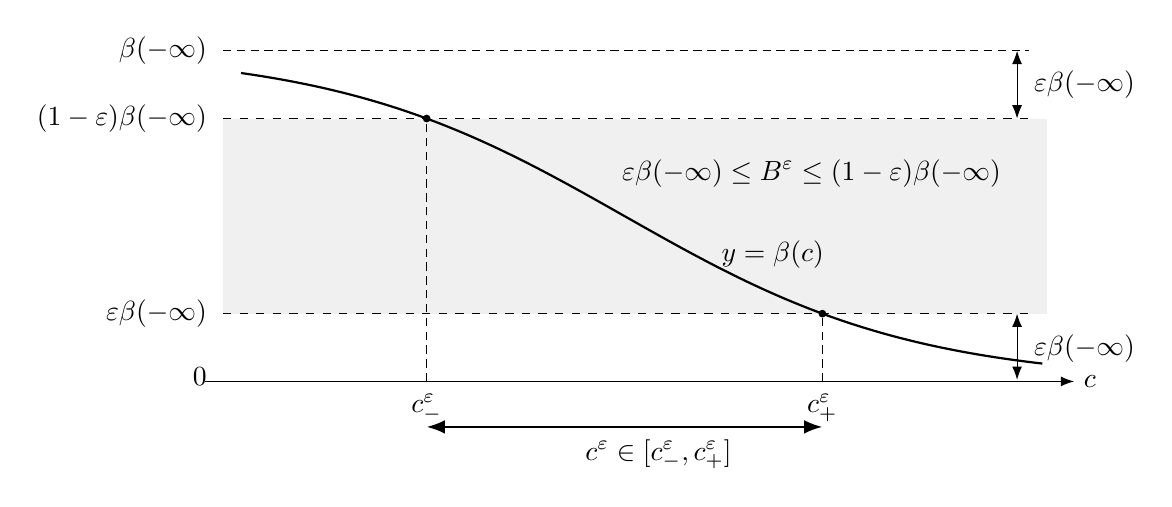
\begin{tikzpicture}[x=1.15cm,y=1.05cm,>=Latex]
  % admissible strip
  \fill[black!6] (-4.75,0.82) rectangle (4.35,3.18);

  % axes
  \draw[->] (-4.95,0) -- (4.65,0) node[right] {$c$};
  % \draw[->] (-1.00,-0.05) -- (-1.00,4.55) node[above] {$\beta(c)$};

  % beta curve (schematic)
  \draw[thick,domain=-4.55:4.30,samples=100,smooth,variable=\x]
  plot
  ({\x},{4/(1+exp(0.6203*(\x+0.315)))});

\node[anchor=south west] at (0.65,1.25) {$y=\beta(c)$};

  % endpoint and truncation levels
  \draw[densely dashed] (-4.75,4.0) -- (4.15,4.0);
  \draw[dashed] (-4.75,3.18) -- (4.15,3.18);
  \draw[dashed] (-4.75,0.82) -- (4.15,0.82);
  \node[anchor=east] at (-4.82,4.0) {$\beta(-\infty)$};
  \node[anchor=east] at (-4.82,3.18) {$(1-\e)\beta(-\infty)$};
  \node[anchor=east] at (-4.82,0.82) {$\e\beta(-\infty)$};
  \node[anchor=east] at (-4.82,0.06) {$0$};

  % epsilon-sized cuts
  \draw[<->] (4.02,3.18) -- (4.02,4.0);
  \node[anchor=west] at (4.10,3.59) {$\e\beta(-\infty)$};
  \draw[<->] (4.02,0.02) -- (4.02,0.82);
  \node[anchor=west] at (4.10,0.40) {$\e\beta(-\infty)$};

  % inverse images of truncation levels
  \draw[densely dashed] (-2.50,0) -- (-2.50,3.18);
  \draw[densely dashed] (1.87,0) -- (1.87,0.82);
  \fill (-2.50,3.18) circle (1.4pt);
  \fill (1.87,0.82) circle (1.4pt);
  \node[anchor=north] at (-2.50,-0.04) {$c_-^\e$};
  \node[anchor=north] at (1.87,-0.04) {$c_+^\e$};

  % compact c interval and strip label
  \draw[<->,thick] (-2.50,-0.55) -- (1.87,-0.55);
  \node at (0.06,-0.88) {$c^\e\in[c_-^\e,c_+^\e]$};
  \node[align=center] at (1.75,2.52)
    {$\e\beta(-\infty)\leq B^\e\leq(1-\e)\beta(-\infty)$};
\end{tikzpicture}
\caption{Schematic range regularization of the degeneracy parameter.  The truncation keeps $B^\e$ in a compact subinterval of $(0,\beta(-\infty))$, equivalently keeping $c^\e=\beta^{-1}(B^\e)$ in a compact interval.}
\label{fig:Beps-cons}

 

\end{figure}


Finally, when $N>0$, we set
\begin{equation}\label{eq/areg}
a^\e:=\beta_0(c^\e)^{\frac23}(N^\e)^{-\frac23}
\end{equation}
and
\bq \label{eq:Feps}
 \calF^\e(f)(p) :=\frac1{e^{a^\e|p-u^\e|^2+c^\e}+\hbar}.
\eq
If $N=0$, define $\calF^\e(f)=0$.  This last convention is consistent with the limit $N^\e\downarrow0$ in $L^1(\R^3_p)$.



The range truncation and the vacuum interpolation play complementary roles. The former controls the inverse moment map, while the latter removes the singularity at vacuum without losing uniform moment control. In particular, the regularization acts at the level of the macroscopic parameters, so that the approximate profile remains within the Fermi--Dirac family. Exact moment matching is not imposed at this stage: by \eqref{eq:FD-mom-com},
\bq \label{eq:Feps-mom}
 N_{\calF^\e(f)}=N^\e,\quad  P_{\calF^\e(f)}=N^\e u^\e,\quad  E_{\calF^\e(f)}=(\be)^{-\frac53}(N^\e)^{\frac53}  +N^\e|u^\e|^2.
\eq


\begin{remark} 
The interpolation near vacuum is introduced not merely to remove the degeneracy of the parametrization, but also to retain control of the equilibrium moments in terms of the input moments. For example, simply replacing $S^\e$ by $S^\e+\e$ and setting
\[
 B_{\rm add}^\e:=\frac{N}{(S^\e+\e)^{\frac35}}
\]
would give
\[
 (B_{\rm add}^\e)^{-\frac53}(N^\e)^{\frac53}
 =
 \frac{S^\e+\e}{(1+\e N)^{\frac53}}.
\]
For fixed $\e>0$, this quantity tends to $\e$, rather than to zero, as $(N,P,E)$ approaches vacuum through $N>0$. Hence this regularization alone does not yield an estimate of the form
\[
 E_{\calF^\e(f)}\le C_\hbar(N_f+E_f),
\]
which is needed uniformly in $\e$ for the compactness argument.

The interpolation in the definition of $B^\e$ avoids this nonvanishing energy contribution near vacuum while retaining the lower bound on $B^\e$ required for the uniform moment estimate below.
\end{remark}


\begin{lemma}\label{lem:unif-e}
There is a constant $C_\hbar>0$, independent of $\e\in(0,\frac12)$ and of $f$, such that every Pauli-admissible $f$ satisfies
\[
 \int_{\R^3}(1+|p|^2)\calF^\e(f)(p)\,\dpp  \leq C_\hbar(N_f+E_f).
\]
\end{lemma}

\begin{proof}
By Lemma \ref{lem:sharp-pauli}, whenever $N>0$,
\begin{equation}\label{eq/ easy}
 \frac{N}{(N+E)^{\frac35}}  \leq \frac{N}{(E-|P|^2/N)^{\frac35}}  \leq\beta(-\infty).
\end{equation}
The assertion is trivial if $N=0$.  From \eqref{eq:S-bds},
\[%\begin{equation}\label{eq/ wtB low}
 \widetilde B^\e  \geq(1+\e)^{-\frac35}\frac{N}{(N+E)^{\frac35}}.
\]%\end{equation}
The upper truncation value satisfies, simply because of \eqref{eq/ easy},
\[
 (1-\e)\beta(-\infty) \geq\frac12\frac{N}{(N+E)^{\frac35}}.
\]
Together, we see that the range-truncated $\overline{B^\e}$, and then also the convex combination $\be$, satisfy
\bq \label{eq:B-lower}
 \be(N,P,E)  \geq C_0\frac{N}{(N+E)^{\frac35}}
\eq
with a universal $C_0>0$, independent of $\e\in(0,\frac12)$.

Using \eqref{eq:Feps-mom}, $N^\e\leq N$, and \eqref{eq:B-lower},
\[
 (\be)^{-\frac53}(N^\e)^{\frac53}  \leq C(N+E).
\]
Moreover, for $N>0$, $|u^\e|\leq\frac{|P|}{N}$, and thus
\begin{equation}\label{eq:E-lower}
 N^\e|u^\e|^2 \leq\frac{|P|^2}{N}\leq E.
\end{equation}
This together with the following identity
\[
 \int_{\R^3}(1+|p|^2)\calF^\e(f)(p)\,\dpp = N^\e + (\be)^{-\frac53}(N^\e)^{\frac53} +  N^\e|u^\e|^2
\]
gives the desired result.  The case $N=0$ is immediate from the definition. This completes the proof.
\end{proof}

For fixed $\e>0$, the regularization also restores the Lipschitz property required for the Picard construction.


\begin{lemma}\label{lem:fix-e-Lip}
For each fixed $\e\in(0,\frac12)$, there exists $C_{\e,\hbar}<\infty$ such that, whenever $f,g$ are Pauli-admissible,
\[
 \|\calF^\e(f)-\calF^\e(g)\|_{L^1_2(\R^3_p)} \leq C_{\e,\hbar}\|f-g\|_{L^1_2(\R^3_p)}.
\]
\end{lemma}

\begin{proof}
If $N_f=0$ or $N_g=0$, then the assertion becomes trivial due to \eqref{eq:Feps-mom},  $N^\e\leq N$, and \eqref{eq:E-lower}. Let $N_f$ and $N_g$ be non-zero and set 
\[
 (N,P,E):=(N_f,P_f,E_f),  \quad  (N',P',E'):=(N_g,P_g,E_g).
\]
Since
\[
 |N-N'|+|P-P'|+|E-E'| \leq C\|f-g\|_{L^1_2(\R^3_p)},
\]
it suffices to establish Lipschitz dependence of the regularized parameters on the moments and then of the Fermi--Dirac profile on these parameters.

From \eqref{eq:reg-N-u},
\[
 |N_f^\e-N_g^\e|  =\frac{|N-N'|}{(1+\e N)(1+\e N')}  \leq |N-N'|.
\]
For the regularized velocity, set
\[
 d:=N+\e(1+|P|),  \quad  d':=N'+\e(1+|P'|).
\]
Since $d,d'\geq\e$ and $|P'|/d'\leq\frac1\e$, we obtain
\begin{align*}
 |u_f^\e-u_g^\e|  &\leq  \frac{|P-P'|}{d}  +\frac{|P'|}{d'}\frac{|d-d'|}{d} \\
 &\leq  \frac1\e|P-P'|  +\e^{-2}\lt(|N-N'|+\e|P-P'|\rt) \\
 &\leq  \e^{-2}|N-N'|  +2\frac1\e|P-P'|.
\end{align*}

We next estimate the regularized degeneracy parameter $B^\e$. On the region $N+E\geq\e$, write
\[
 D^\e=(1+\e)N+\e E,  \quad  S^\e  =E-\frac{|P|^2}{D^\e}+\e(N+E).
\]
The physical moment inequality $ |P|^2\leq NE$ implies
\[
 |P|\leq\sqrt{NE}\leq\frac{N+E}{2},
\]
while
\[
 D^\e\geq\e(N+E),  \quad  S^\e\geq\e(N+E)\geq\e^2.
\]
A direct differentiation gives
\[
 \pa_N S^\e  =  \frac{(1+\e)|P|^2}{(D^\e)^2}+\e,  \quad  \nabla_P S^\e  =  -\frac{2P}{D^\e}, \quad  \pa_E S^\e  =  1+\e+\frac{\e|P|^2}{(D^\e)^2}.
\]
Using these bounds, we find
\bq \label{eq:Seps-deri-bd}
 |\pa_N S^\e|  +|\nabla_P S^\e|  +|\pa_E S^\e|  \leq C_\e  \quad\text{on }\{N+E\geq\e\}.
\eq

Since $N\leq N+E\leq\frac1\e S^\e$, differentiating $\widetilde B^\e  =N(S^\e)^{-\frac35}$ yields
\[
 \pa_N\widetilde B^\e   =  (S^\e)^{-\frac35}  -\frac35N(S^\e)^{-8/5}\pa_NS^\e,\quad \nabla_P\widetilde B^\e =  -\frac35N(S^\e)^{-8/5}\nabla_PS^\e,\quad  \pa_E\widetilde B^\e =  -\frac35N(S^\e)^{-8/5}\pa_ES^\e.
\]
Hence \eqref{eq:Seps-deri-bd}, together with $S^\e\geq\e^2$, gives
\bq \label{eq:Btilde-deri-bd}
 |\pa_N\widetilde B^\e|  +|\nabla_P\widetilde B^\e|  +|\pa_E\widetilde B^\e|  \leq C_\e  \quad\text{on }\{N+E\geq\e\}.
\eq

The max--min maps used in the range truncation \eqref{eq:Bhat} are one-Lipschitz.  In the transition region $ \e\leq N+E\leq2\e$, we also have
\[
 |\chi_\e'|\leq\frac{C}{\e},
\]
while both $\overline{B^\e}$ and $(1-\e)\beta(-\infty)$ are bounded by constants depending only on $\e$ and $\hbar$.  On $N+E\leq\e$, the function $B^\e$ is constant.   Together with \eqref{eq:Btilde-deri-bd}, this yields a bound $C_{\e,\hbar}$ for the derivatives of $B^\e$ wherever they exist.

Now let
\[
 Z_\theta  :=  (1-\theta)(N,P,E)+\theta(N',P',E'),  \quad 0\leq\theta\leq1.
\]
Since $Z_\theta$ is the moment triple of $(1-\theta)f+\theta g$, the whole segment remains in the physical moment set.  Integrating the derivative bound along this segment, piecewise across the truncation interfaces, gives
\bq\label{eq:Beps-L-mom}
 |B^\e(N,P,E)-B^\e(N',P',E')|  \leq C_{\e,\hbar}  \lt(|N-N'|+|P-P'|+|E-E'|\rt).
\eq

By \eqref{eq:Beps-range},
\[
 c^\e\in I_\e  :=  \lt[  \beta^{-1}((1-\e)\beta(-\infty)),  \beta^{-1}(\e\beta(-\infty))  \rt].
\]
Since $\beta'$ is continuous and strictly negative,
\[
 \inf_{c\in I_\e}|\beta'(c)|>0,
\]
and hence the inverse function theorem gives
\[
 |\beta^{-1}(z)-\beta^{-1}(z')|  \leq C_{\e,\hbar}|z-z'| \quad \text{for } z,z'\in[\e\beta(-\infty),(1-\e)\beta(-\infty)].
\]
Combining this with \eqref{eq:Beps-L-mom}, we obtain
\[
 |c_f^\e-c_g^\e|  \leq C_{\e,\hbar}  \lt(  |N-N'|+|P-P'|+|E-E'|  \rt).
\]

It remains to estimate the dependence of the Fermi--Dirac profile on these regularized parameters.  For $N>0$, $c\in I_\e$, and $u\in\R^3$, define
\[
 \Phi(N,c,u)(p)  :=  \frac1{  \exp\lt(\beta_0(c)^{\frac23}N^{-\frac23}|p-u|^2+c\rt)  +\hbar}.
\]
Due to the definition of $\calF^\e$, we only need consider parameters satisfying
\[
 0<N\leq\frac1\e,  \quad  |u|\leq\frac1\e.
\]
Set
\[
 Q  :=  \beta_0(c)^{\frac23}N^{-\frac23}|p-u|^2+c,  \quad  \Lambda(Q)  :=  \frac{e^Q}{(e^Q+\hbar)^2}.
\]
A direct differentiation gives
\begin{equation}\label{eq/ dir diff}
\begin{aligned}
 \pa_N\Phi  &=  \frac23\Lambda(Q)  \beta_0(c)^{\frac23}N^{-\frac53}|p-u|^2,\quad  \nabla_u\Phi  =  2\Lambda(Q)  (\beta_0(c))^{\frac23}N^{-\frac23}(p-u),\\
 \pa_c\Phi  &=  -\Lambda(Q)  \lt(  1+  \frac23\frac{\beta_0'(c)}{\beta_0(c)}  (\beta_0(c))^{\frac23}N^{-\frac23}|p-u|^2  \rt).
\end{aligned}
\end{equation}

We now claim that
\bq \label{eq:Phi-deri}
 \|\pa_N\Phi\|_{L^1_2(\R^3_p)}  +\|\nabla_u\Phi\|_{L^1_2(\R^3_p)}  +\|\pa_c\Phi\|_{L^1_2(\R^3_p)}  \leq C_{\e,\hbar}.
\eq
Indeed, making the change of variables
\[
 p  =  u+N^{\frac13}\beta_0(c)^{-\frac13}v,  \quad  \dpp  =  N\beta_0(c)^{-1}\,\dd v,
\]
we have
\[
 Q=|v|^2+c \quad \text{and} \quad N^{-\frac53} |p-u|^2 \,\dpp = \beta_0(c)^{-\frac{5}{3}} |v|^2 \, \mathrm{d}v.
\]
Thus, after the above change of variables, the $N$-factors in the integrals of \eqref{eq/ dir diff} are respectively of order $1$, $N^{\frac23}$, and $N$. Moreover, since $c\in I_\e$, both $\beta_0(c)$ and $\beta_0'(c)/\beta_0(c)$ are uniformly bounded on $I_\e$, with $\beta_0(c)$ bounded away from zero; further, $|u|\leq\frac1\e$, and $\Lambda(|v|^2+c)$ has Gaussian decay uniformly for $c\in I_\e$. This proves \eqref{eq:Phi-deri}. In particular, the estimate for $\pa_N\Phi$ remains uniform as $N\downarrow0$, while the other two terms vanish in that limit; so $\Phi$ extends continuously to $N=0$ by setting
\[
 \Phi(0,c,u):=0.
\]


Integrating the derivative bounds in \eqref{eq:Phi-deri} successively along the $N$-, $c$-, and $u$-segments, we obtain
\[
 \|\Phi(N,c,u)-\Phi(N',c',u')\|_{L^1_2(\R^3_p)}  \leq  C_{\e,\hbar}  \lt(  |N-N'|+|c-c'|+|u-u'|  \rt).
\]
Since
\[
 \calF^\e(f)  =  \Phi(N_f^\e,c_f^\e,u_f^\e),  \quad  \calF^\e(g)  =  \Phi(N_g^\e,c_g^\e,u_g^\e),
\]
combining all of the above estimates yields the desired result.
\end{proof}

%%%%%%%%%%%%%%%%%%%%%%%%%%%%%%%%%%%%%%%%%%%%%%%
%
%
%
%
%
%
%%%%%%%%%%%%%%%%%%%%%%%%%%%%%%%%%%%%%%%%%%%%%%%

\subsection{The equilibrium map on the admissible moment set}\label{sec:ext-equil}

 In this section, we investigate the consistency of the regularization $\calF^\e$ as $\e\downarrow 0$. Toward this end, we need to first show that it is possible to match, to each Pauli-admissible $f$, a unique local equilibrium $\calF(f)$ which is determined by its moments. As we will see, the ordinary Fermi-Dirac distribution will be its interior representation, whereas its saturated form will be the boundary representation.

Indeed, for $N>0$, set
\[
 E_\star(N,P):=\frac{|P|^2}{N}+\kappah N^{\frac53}
\]
and define the non-vacuum admissible moment set
\[
 \mathfrak M_\hbar :=\{(N,P,E):N>0,\ E \ge E_\star(N,P)\}.
\] 
By Lemma \ref{lem:sharp-pauli}, every non-vacuum moment triple arising from a function satisfying the Pauli bound and having finite second moments belongs to $\mathfrak M_\hbar$.  Conversely, Proposition \ref{prop:vari} below constructs a Pauli-admissible distribution for every triple in $\mathfrak M_\hbar$.  The vacuum triple is $(0,0,0)$; it will always be handled separately by setting the local equilibrium equal to zero.

For $(N,P,E)\in\mathfrak M_\hbar$, let
\[
 \calC_\hbar(N,P,E)  :=\lt\{  g: 0\leq g\leq\frac1\hbar ,\ (1+|p|^2)g\in L^1(\R^3),\  \int_{\R^3}(1,p,|p|^2)g\,\dpp=(N,P,E)  \rt\}.
\]
We also recall the Fermi-Dirac entropy density
\[
 \eta_\hbar(z) =z\log z+\frac1\hbar(1-\hbar z)\log(1-\hbar z),  \quad 0\leq z\leq\frac1\hbar ,
\]
with the convention $0\log0=0$. Now using the preceding moment characterization, let us define the exact equilibrium intrinsically, including the saturation boundary, as the unique minimizer of the Fermi-Dirac entropy.


\begin{proposition}\label{prop:vari}
For every $(N,P,E)\in\mathfrak M_\hbar$, the problem
\[
 \inf_{g\in\calC_\hbar(N,P,E)}  \int_{\R^3}\eta_\hbar(g(p))\,\dpp
\]
has a unique minimizer, denoted by $\calF[N,P,E]$.  If $E>E_\star(N,P)$, then
\bq \label{eq:inte-FD}
 \calF[N,P,E](p)  =\frac1{e^{a|p-u|^2+c}+\hbar},  \quad  u=\frac PN,
\eq
where $c\in\R$ and $a>0$ are determined by
\[
 \beta(c)=B(N,P,E),  \quad  a=\beta_0(c)^{\frac23}N^{-\frac23}.
\]
If $E=E_\star(N,P)$, then
\bq \label{eq:satu-FD}
 \calF[N,P,E](p)  =\frac1\hbar\one_{\{|p-P/N|\leq R_N\}},  \quad  R_N=\lt(\frac{3\hbar N}{4\pi}\rt)^{\frac13}.
\eq
In both cases,
\[
 \int_{\R^3}(1,p,|p|^2)\calF[N,P,E](p)\,\dpp=(N,P,E).
\]
\end{proposition}

\begin{proof}
By Lemma \ref{lem:sharp-pauli} and \eqref{eq:beta-kappa},
\[
 E\geq E_\star(N,P)  \quad\Longleftrightarrow\quad  B(N,P,E)\leq\beta(-\infty).
\]
Assume first that $E>E_\star(N,P)$.  Lemma \ref{lem:beta} gives a unique $c\in\R$ satisfying $\beta(c)=B(N,P,E)$.  Let $F$ denote the function in \eqref{eq:inte-FD}.  With
\[
 p=u+N^{\frac13}\beta_0(c)^{-\frac13}v,
\]
the moment identities \eqref{eq:FD-mom-com}--\eqref{eq:FD-mom} give
\[
 \int_{\R^3}F\,\dpp=N,  \quad  \int_{\R^3}pF\,\dpp=P,
\]
and
\[
 \int_{\R^3}|p|^2F\,\dpp  =\beta(c)^{-\frac53}N^{\frac53}+N|u|^2=E.
\]
Thus $F\in\calC_\hbar(N,P,E)$.

For $z\in(0,\frac1\hbar )$,
\[
 \eta_\hbar'(z)=\log\frac{z}{1-\hbar z},  \quad  \eta_\hbar''(z)=\frac1{z(1-\hbar z)}>0.
\]
Moreover,
\[
 \eta_\hbar'(F(p))=-a|p-u|^2-c,
\]
which is a linear combination of $1,p_1,p_2,p_3,|p|^2$.  Hence, for every $g\in\calC_\hbar(N,P,E)$, convexity gives
\[
 \int_{\R^3}\lt(\eta_\hbar(g)-\eta_\hbar(F)\rt)\,\dpp \geq\int_{\R^3}\eta_\hbar'(F)(g-F)\,\dpp =0.
\]
The integrals are finite. For the second term in the entropy density,
\[
 -z\leq\frac1\hbar(1-\hbar z)\log(1-\hbar z)\leq0,
\]
while, with $V(p)=1+|p|^2$,
\[
 z\log z=z\log(ze^V)-Vz\geq-e^{-V-1}-Vz,
\]
and $(z\log z)^+\leq C_\hbar z$ on $[0,\frac1\hbar ]$.  Strict convexity yields uniqueness.

If $E=E_\star(N,P)$, Lemma \ref{lem:sharp-pauli} shows that $\calC_\hbar(N,P,E)$ consists of the single function in \eqref{eq:satu-FD}.  This completes the proof.
\end{proof}

For a Pauli-admissible function $f=f(p)$ with finite local second moments, define
\[
 \calF(f)(p)  :=\calF[N_f,P_f,E_f]  \quad\text{when }N_f>0,
\]
and set $\calF(f)=0$ when $N_f=0$. The latter definition is consistent since nonnegativity and zero mass imply $f\equiv 0$ almost everywhere. In the case where $f$ is dependent also on time and space, we define $\calF(f)(t,x,p)$ pointwisely for each $(t,x)$ in the natural way. 


To analyze the equilibrium map near the saturation boundary, we need the asymptotic behavior of the finite-temperature parameters as $c\to-\infty$.  Indeed, approaching $B(N,P,E)=\beta(-\infty)$ from the interior corresponds precisely to this zero-temperature regime.  The following asymptotics will identify the limiting Fermi radius.

\begin{lemma}\label{lem:beta0-ze-t}
As $C\to+\infty$,
\[
 \beta_0(-C)=\frac{4\pi}{3\hbar}C^{\frac32}(1+o(1)), \quad \beta_2(-C)=\frac{4\pi}{5\hbar}C^{\frac52}(1+o(1)).
\]
\end{lemma}

\begin{proof}
With $p=\sqrt C\,q$,
\[
 C^{-\frac32}\beta_0(-C)  =4\pi\int_0^\infty\frac{r^2}{e^{C(r^2-1)}+\hbar}\,\dr.
\]
On $r\in(0,1)$ the integrand is bounded by $\frac1\hbar r^2$ and converges to that function.  On $(1,\infty)$, for $C\geq1$,
\[
 \frac{r^2}{e^{C(r^2-1)}+\hbar}  \leq r^2e^{-(r^2-1)},
\]
which is integrable.  Dominated convergence gives the first asymptotic formula.  The same argument, with $r^4$ in place of $r^2$, gives the second assertion.
\end{proof}

We now state for later use an elementary form of Scheff\'e's lemma, which will be used repeatedly.

\begin{lemma} \label{lem:pos-L1}
Let $(X,\mu)$ be a measure space and let $h_j,h\geq0$ belong to $L^1(X,\mu)$.  If $h_j\to h$ almost everywhere and
\[
 \int_X h_j\,\dd\mu \to \int_X h\,\dd\mu,
\]
then $h_j\to h$ strongly in $L^1(X,\mu)$.
\end{lemma}

\begin{proof}
Since $\min\{h_j,h\}\to h$ almost everywhere and $0\leq\min\{h_j,h\}\leq h$, dominated convergence gives
\[
 \int_X \min\{h_j,h\} \, \dd\mu \to \int_X h\,\dd\mu.
\]
The identity
\[
 \int_X |h_j-h|\,\dd\mu  =\int_X h_j\,\dd\mu+\int_X h\,\dd\mu  -2\int_X \min\{h_j,h\}\,\dd\mu
\]
proves the claim.
\end{proof}


The following proposition is unrelated to the regularization, but of independent interest. It shows that we can prove continuity of the exact equilibrium map, on the entire admissible moment set. The nonstandard point is continuity at the saturation boundary, where the finite-temperature parameter $c$ tends to $-\infty$. Lemma \ref{lem:beta0-ze-t} identifies the pointwise limit, while Lemma \ref{lem:pos-L1} upgrades it to strong weighted $L^1$ convergence.

\begin{proposition}%\label{prop:conti}
Let $(N_j,P_j,E_j),(N,P,E)\in\mathfrak M_\hbar$ and assume
\begin{equation}\label{eq/ mom conv}
 (N_j,P_j,E_j)\to(N,P,E).
\end{equation}
Then
\bq \label{eq:conti}
 \calF[N_j,P_j,E_j]  \to \calF[N,P,E]  \quad\text{strongly in }L^1_2(\R^3_p).
\eq
\end{proposition}

\begin{proof}
Set $F_j=\calF[N_j,P_j,E_j]$ and $F=\calF[N,P,E]$. Proposition \ref{prop:vari} and the assumption \eqref{eq/ mom conv} already tell us that
\[
 \int_{\R^3}(1+|p|^2)F_j\,\dpp=N_j+E_j  \to N+E  =\int_{\R^3}(1+|p|^2)F\,\dpp.
\]
In view of Lemma \ref{lem:pos-L1} it therefore suffices to check that $F_j(p)\to F(p)$ a.e., and \eqref{eq:conti} would be proven.
 

Assume that $E>E_\star(N,P)$. Then eventually $E_j>E_\star(N_j,P_j)$, and continuity of $\beta^{-1}$ on $(0,\beta(-\infty))$ gives
\[
 c_j\to c,  \quad  u_j=\frac{P_j}{N_j}\to\frac PN,  \quad  a_j\to a.
\]
Thus $F_j(p)\to F(p)$ for every $p$ and we obtain \eqref{eq:conti}.

Assume now that $E=E_\star(N,P)$.  For indices satisfying $E_j=E_\star(N_j,P_j)$, the profiles are saturated distributions: $F_j(p) = \mathbf{1}_{|p-P_j/N_j|\le R_{N_j}}$. Since $P_j/N_j\to P/N$ and $R_{N_j}\to R_N$, clearly $F_j(p)$ is a.e. convergent to $F(p)$ and we are done. Next, it remains to prove convergence for the indices where $E_j > E_\star(N_j,P_j)$. By assumption,
\[
 B(N_j,P_j,E_j)\to\beta(-\infty),
\]
and thus $c_j\to-\infty$.  Set  
\[
C_j=-c_j \quad \text{and} \quad r_j^2:=\frac{C_j}{a_j}.
\]
By Lemma \ref{lem:beta0-ze-t},
\[
 r_j^3  =\frac{C_j^{\frac32}N_j}{\beta_0(-C_j)}  \to\frac{3\hbar N}{4\pi}=R_N^3.
\]
Hence $r_j\to R_N$, $u_j\to u=P/N$, and $a_j=C_j/r_j^2\to+\infty$.  Since
\[
 a_j|p-u_j|^2+c_j  =a_j\lt(|p-u_j|^2-r_j^2\rt),
\]
we obtain for every $p$ with $|p-u|\neq R_N$,
\[
 F_j(p)\to\frac1\hbar\one_{\{|p-u|<R_N\}}=F(p)  \quad\text{a.e. in }p.
\]
This completes the proof.
\end{proof}

In particular, if a sequence of admissible moment triples converges to the vacuum triple $(0,0,0)$, the corresponding exact equilibria converge to zero immediately, since
\[
 \|\calF[N_j,P_j,E_j]\|_{L^1_2(\R^3_p)}=N_j+E_j\to0.
\]

The next proposition is the one that is of practical use to us, as it gives the consistency of the $\e$-regularization with respect to the exact equilibrium. Note carefully that the argument of the regularized Fermi-Dirac distribution is also assumed to change with the parameter $\e$. Indeed, this is the form needed later in the compactness argument. Convergence of the macroscopic moments determines the strong limit of the regularized equilibrium profile throughout the admissible moment set, including the saturation boundary.

\begin{proposition}\label{prop:consist}
Let $\e_j\downarrow0$, and let $(N_j,P_j,E_j)$ be moment triples generated by Pauli-admissible functions $\{f_j\}$. We assume
\[
 (N_j,P_j,E_j)\to(N,P,E),
\]
where either $(N,P,E)\in\mathfrak M_\hbar$ or $(N,P,E)=(0,0,0)$. Let $F_j^{\rm reg} := \calF^{\e_j}(f_j)$ be the regularized profile obtained by \eqref{eq:reg-N-u}--\eqref{eq:Feps}, with $\e=\e_j$. Then
\bq \label{eq:consi}
 F_j^{\rm reg}\to\calF[N,P,E] \quad\text{strongly in }L^1_2(\R^3_p),
\eq
where $\calF[0,0,0]:=0$.
\end{proposition}

\begin{proof}
Throughout this proof let us denote by $N_j^{\e_j},u_j^{\e_j},c^{\e_j}_j,\ldots$ the quantities defined through \eqref{eq:reg-N-u}--\eqref{eq/areg}, by using $(N_j,P_j,E_j)$ in place of $(N,P,E)$.

If $(N,P,E)=(0,0,0)$, Lemma \ref{lem:unif-e} gives
\[
 \|F_j^{\rm reg}\|_{L^1_2(\R^3_p)}  \leq C_\hbar(N_j+E_j)\to0.
\]
Assume from now on that $N>0$. Since $N_j\to N$, eventually $N_j\geq N/2$, and so
\bq \label{eq:consi-Nu}
 N_j^{\e_j}=\frac{N_j}{1+\e_jN_j}\to N,  \quad  u_j^{\e_j}=\frac{P_j}{N_j+\e_j(1+|P_j|)}\to\frac PN.
\eq
Moreover, $\chi_{\e_j}(N_j+E_j)=1$ for all sufficiently large $j$, and
\[
 S_j^{\e_j} =E_j-\frac{|P_j|^2}{N_j+\e_j(N_j+E_j)}    +\e_j(N_j+E_j) \to E-\frac{|P|^2}{N}.
\]
Hence $\widetilde B_j^{\e_j}\to B(N,P,E)$.  Since the lower and upper truncation levels tend to $0$ and $\beta(-\infty)$, respectively,
\bq \label{eq:consi-B}
 B_j^{\e_j}\to B(N,P,E).
\eq

Let us consider two cases separately. If $B(N,P,E)<\beta(-\infty)$, then by continuity of $\beta^{-1}$ on $(0,\beta(-\infty))$, we deduce from \eqref{eq:consi-B} that $c^{\e_j}_j \to c = \beta^{-1}(B(N,P,E))$. Combining this with \eqref{eq:consi-Nu}, we obtain 
\[
 F_j^{\rm reg}(p)\to\calF[N,P,E](p).
\]
Furthermore, from \eqref{eq:Feps-mom} and \eqref{eq:consi-Nu}:
\[
 \int_{\R^3}(1+|p|^2)F_j^{\rm reg}\,\dpp =N_j^{\e_j}  +(B_j^{\e_j})^{-\frac53}(N_j^{\e_j})^{\frac53}  +N_j^{\e_j}|u_j^{\e_j}|^2 \to N+E.
\]
Applying Lemma \ref{lem:pos-L1} with $\mathrm{d}\mu=(1+|p|^2)\dpp$ proves \eqref{eq:consi}.

Suppose finally that $B(N,P,E)=\beta(-\infty)$. Then \eqref{eq:consi-B} shows $c_j^{\e_j}=\beta^{-1}(B_j^{\e_j})\to-\infty$.  Set  
\[
C_j=-c_j^{\e_j} \quad \text{and} \quad  r_j^2:=\frac{C_j}{a_j^{\e_j}}.
\]
Since $a_j^{\e_j}  =\beta_0(-C_j)^{\frac23}(N_j^{\e_j})^{-\frac23}$, Lemma \ref{lem:beta0-ze-t} and \eqref{eq:consi-Nu} give
\[
 r_j^3  =\frac{C_j^{\frac32}N_j^{\e_j}}{\beta_0(-C_j)}  \to\frac{3\hbar N}{4\pi}=R_N^3.
\]
Thus the profiles converge pointwise away from $|p-P/N|=R_N$ to the saturated equilibrium \eqref{eq:satu-FD}.  Their weighted integrals converge to
\[
 N+\beta(-\infty)^{-\frac53}N^{\frac53}+N\lt|\frac PN\rt|^2=N+E,
\]
thanks to the preceding moment formula and by recalling the assumption $B(N,P,E)=\beta(-\infty)$. A final application of Lemma \ref{lem:pos-L1} proves \eqref{eq:consi}.
\end{proof}

%%%%%%%%%%%%%%%%%%%%%%%%%%%%%%%%%%%%%%%%%%%%%%%
%
%
%
%
%
%
%%%%%%%%%%%%%%%%%%%%%%%%%%%%%%%%%%%%%%%%%%%%%%%

\subsection{The regularized equation}

For fixed $\e\in(0,\frac12)$, consider
\bq \label{eq:reg-PDE}
\pa_t f^\e+p\cdot\nabla_xf^\e  =\calF^\e(f^\e)-f^\e,  \quad  f^\e|_{t=0}=f_0.
\eq

The preceding growth and Lipschitz estimates allow us to solve the regularized equation by Picard iteration on arbitrary finite time intervals.


\begin{proposition}\label{prop:regul-exi}
Under \eqref{eq:ini}, for every fixed $\e\in(0,\frac12)$ there exists
\[
 f^\e\in C([0,\infty);L^1_2(\R^3 \times \R^3))
\]
satisfying
\bq \label{eq:reg-mild}
 f^\e(t,x,p)  =e^{-t}f_0(x-tp,p)  +\int_0^t e^{-(t-s)}  \calF^\e(f^\e)(s,x-(t-s)p,p)\,\ds.
\eq
Moreover,
\bq \label{eq:reg-pauli}
 0\leq f^\e\leq\frac1\hbar ,
\eq
and, for every $T>0$,
\bq \label{eq:unif-f-eps}
 \sup_{0<\e<\frac12}\sup_{0\leq t\leq T}  \|f^\e(t)\|_{L^1_2}\leq C_{T,\hbar,f_0}.
\eq
The same bound holds for $\calF^\e(f^\e)$ in place of $f^\e$.
\end{proposition}

\begin{proof}
Fix $\e\in(0,\frac12)$ and $T>0$. We construct the solution directly on $[0,T]$ by Picard iteration. Set
\[
 f^{0,\e}(t,x,p):=e^{-t}f_0(x-tp,p),
\]
and define recursively
\bq \label{eq:reg-Picard}
 f^{n+1,\e}(t,x,p) =e^{-t}f_0(x-tp,p) +\int_0^t e^{-(t-s)}  \calF^\e(f^{n,\e})(s,x-(t-s)p,p)\,\ds,  \quad n\geq0.
\eq
Since $0\leq\calF^\e(g)\leq\frac1\hbar $, induction gives
\[
 0\leq f^{n+1,\e}(t,x,p) \leq e^{-t}\frac1\hbar   +\frac1\hbar \int_0^t e^{-(t-s)}\,\ds =\frac1\hbar .
\]
The strong continuity of free transport in $L^1_2$, together with Lemmas \ref{lem:unif-e} and \ref{lem:fix-e-Lip}, shows inductively that every iterate belongs to $C([0,T];L^1_2)$. Moreover,
\[
 \sup_{0\leq t\leq T}\|f^{1,\e}(t)-f^{0,\e}(t)\|_{L^1_2} \leq C_\hbar T\|f_0\|_{L^1_2}.
\]
For $n\geq1$, applying Lemma \ref{lem:fix-e-Lip} to the difference between the iteration formulas for $f^{n+1,\e}$ and $f^{n,\e}$, and using the change of variables $y=x-(t-s)p$, which preserves the weight $1+|p|^2$, we obtain, for any $T>0$ and $t\in[0,T]$,
	\begin{align*}
		\|f^{n+1,\e}(t)-f^{n,\e}(t)\|_{L^1_2}&\leq C_{\e,\hbar}\int_0^t e^{-(t-s_1)}  \|f^{n,\e}(s_1)-f^{n-1,\e}(s_1)\|_{L^1_2}\,\ds_1 \\
		&\leq C_{\e,\hbar}^n\int_0^t\cdots \int_0^{s_{n-1}}   \|f^{1,\e}(s_n)-f^{0,\e}(s_n)\|_{L^1_2}\,\ds_n\cdots \ds_1 \\
		&\le C_{\hbar,f_0,T}\frac{\left(C_{\e,\hbar}t\right)^n}{n!}.
	\end{align*}
Consequently, for $n>m$,
\[
 \sup_{0\le t\le T}  \|f^{n,\e}(t)-f^{m,\e}(t)\|_{L^1_2}  \le C_{\hbar,f_0,T} \sum_{k=m}^{\infty}\frac{(C_{\e,\hbar}T)^k}{k!},
\]
which tends to zero as $m\to\infty$. Hence $\{f^{n,\e}\}_{n\ge0}$ is Cauchy in $C([0,T];L^1_2(\R^3\times\R^3))$.

Let $f^\e\in C([0,T];L^1_2(\R^3\times\R^3))$ denote its limit. The fixed-$\e$ Lipschitz estimate in Lemma \ref{lem:fix-e-Lip} implies
\[
 \calF^\e(f^{n,\e})\to\calF^\e(f^\e)  \quad\text{in }C([0,T];L^1_2(\R^3\times\R^3)),
\]
and therefore we may pass to the limit in \eqref{eq:reg-Picard} to obtain \eqref{eq:reg-mild}. The Pauli bound \eqref{eq:reg-pauli} follows from the corresponding bound for the iterates. Since $T>0$ is arbitrary and the limits agree on overlapping intervals, this defines $f^\e$ globally in time.

It remains to obtain an estimate independent of $\e$.  Lemma \ref{lem:unif-e} and \eqref{eq:reg-mild} give, for $0\leq t\leq T$,
\[
 \|f^\e(t)\|_{L^1_2}  \leq e^{-t}\|f_0\|_{L^1_2}  +C_\hbar\int_0^t e^{-(t-s)}\|f^\e(s)\|_{L^1_2}\,\ds.
\]
Multiplying by $e^t$ and applying Gr\"onwall's inequality yields \eqref{eq:unif-f-eps}.  Lemma \ref{lem:unif-e} gives the same estimate for $\calF^\e(f^\e)$. This completes the proof.
\end{proof}


%%%%%%%%%%%%%%%%%%%%%%%%%%%%%%%%%%%%%%%%%%%%%%%
%
%
%
%
%
%
%%%%%%%%%%%%%%%%%%%%%%%%%%%%%%%%%%%%%%%%%%%%%%%

\section{Compactness and passage to the limit}\label{sec:pass-eps}

Let $\{f^\e\}_{0<\e<\frac12}$ be the family of solutions to the approximating model constructed in Proposition \ref{prop:regul-exi}.  We first establish strong compactness of the density, momentum, and energy fields.  The continuity properties of the moment-to-equilibrium map from Section \ref{sec:ext-equil} then allow us to pass to the nonlinear relaxation term directly from the convergence of these three moments, including at points where the limiting moments lie on the saturation boundary.


%%%%%%%%%%%%%%%%%%%%%%%%%%%%%%%%%%%%%%%%%%%%%%%
%
%
%
%
%
%
%%%%%%%%%%%%%%%%%%%%%%%%%%%%%%%%%%%%%%%%%%%%%%%
\subsection{Compactness of the macroscopic moments}


Our goal in this subsection is to obtain strong compactness of
\[
 (N_{f^\e},P_{f^\e},E_{f^\e}).
\]
Velocity averaging directly gives compactness only for velocity averages with compactly supported test functions.  To reach the physical moments $1$, $p$, and $|p|^2$, we need two additional ingredients: spatial tightness of the density and uniform control of the velocity tails.  We first quantify the mass defect created by the regularization and derive spatial tightness.  We then obtain a local third-moment bound, which provides the additional velocity-tail control required for the energy.


We begin with the total mass. Set
\[
 M^\e(t):=\iint_{\R^3\times\R^3}f^\e(t,x,p)\,\dx\dpp.
\]
Since
\[
 N_{\calF^\e(f^\e)}=\frac{N_{f^\e}}{1+\e N_{f^\e}},
\]
we first derive a quantitative control of the small mass defect generated by the regularization. 
%\textcolor{green}{By the Lebesgue differentiation theorem,  \eqref{eq:reg-mild} gives
%$$	
%\frac{d}{dt}\left\{ f^\e(t,x+vt,v)\right\}= \left\{ \calF^\e(f^\e)-f^\e\right\}(t,x+vt,v)
%$$
%where $f^\e\in  C([0,\infty);L^1_2(\R^3 \times \R^3))$. By \eqref{eq:Feps-mom},  $N^\e_{f^\e}\leq N_{f^\e}$, and \eqref{eq:E-lower}, one finds $\calF^\e(f^\e)\in  C([0,\infty);L^1_2(\R^3 \times \R^3))$ as well. Thus it follows from Tonelli's theorem that
%$$
% \frac{\dd}{\dd t}M^\e(t)  =-\int_{\R^3}\frac{\e N_{f^\e}(t,x)^2}  {1+\e N_{f^\e}(t,x)}\,\dx  \leq0.
% $$
%} 
Let $\zeta_R\in C_c^\infty(\R^3)$ satisfy $0\leq\zeta_R\leq1$, $\zeta_R\uparrow1$, and $|\nabla\zeta_R|\leq C/R$.  Testing \eqref{eq:reg-PDE} against $\zeta_R(x)$ and then letting $R\to\infty$, the transport contribution vanishes since
\[
 \iint_{\R^3\times\R^3}|p|f^\e(t,x,p)\,\dx\dpp  \leq \|f^\e(t)\|_{L^1}^{\frac12}  \lt(\iint_{\R^3\times\R^3}|p|^2f^\e(t,x,p)\,\dx\dpp\rt)^{\frac12},
\]
uniformly on finite time intervals.  Hence
\[
 \frac{\dd}{\dd t}M^\e(t)  =-\int_{\R^3}\frac{\e N_{f^\e}(t,x)^2}  {1+\e N_{f^\e}(t,x)}\,\dx  \leq0.
\]
For $y\geq0$,
\[
 \frac{y}{1+y}\leq y^{\frac23}.
\]
Moreover, by Lemma \ref{lem:sharp-pauli}, we obtain
\[
 \frac{\e N_{f^\e}^2}{1+\e N_{f^\e}}  =N_{f^\e}\frac{\e N_{f^\e}}{1+\e N_{f^\e}}  \leq \e^{\frac23}N_{f^\e}^{\frac53}  \leq \kappah^{-1}\e^{\frac23}E_{f^\e},
\]
and Proposition \ref{prop:regul-exi} gives, for every $T>0$,
\bq \label{eq:m-loss-s}
 0\leq M^\e(0)-M^\e(t)  \leq C_{T,\hbar,f_0}\e^{\frac23},  \quad 0\leq t\leq T.
\eq

Integrating \eqref{eq:reg-PDE} in $p$ gives
\bq \label{eq:den-bal}
\pa_tN_{f^\e}+\nabla_x\cdot P_{f^\e}  =\frac{N_{f^\e}}{1+\e N_{f^\e}}-N_{f^\e}  \leq0.
\eq
Let $\chi_R$ be smooth, equal to zero on $B_R$, equal to one outside $B_{2R}$, and satisfy $|\nabla\chi_R|\leq C/R$.  Testing \eqref{eq:den-bal} by $\chi_R$ gives
\[
 \int_{\R^3}\chi_RN_{f^\e}(t,x)\,\dx  \leq\int_{\R^3}\chi_RN_{f_0}(x)\,\dx  +\frac{C}{R}\int_0^t\int_{\R^3}|P_{f^\e}(s,x)|\,\dx\ds.
\]
The first velocity moment is bounded by mass and kinetic energy, hence Proposition \ref{prop:regul-exi} implies
\bq \label{eq:spa-tig}
 \lim_{R\to\infty}  \sup_{0<\e<\frac12}\sup_{0\leq t\leq T}  \int_{|x|>R}N_{f^\e}(t,x)\,\dx=0.
\eq

The local gain of one velocity moment used below is classical in whole-space BGK compactness arguments; compare \cite{Per89}.  We record the short proof since it also indicates why the estimate is specific to $x\in\R^3$.

\begin{lemma}\label{lem:3-mom}
Let $T,R>0$, and suppose
\[
 f(t,x,p)  =e^{-t}f_0(x-tp,p) +\int_0^te^{-(t-s)}G(s,x-(t-s)p,p)\,\ds,
\]
where $f_0,G\geq0$.  Then
\begin{align*}
 &\int_0^T\int_{B_R}\int_{\R^3}|p|^3f(t,x,p)\,\dpp\dx\dt \\
 &\quad\leq 2R\lt(  \iint_{\R^3\times\R^3}|p|^2f_0(x,p)\,\dx\dpp  +\int_0^T\iint_{\R^3\times\R^3}|p|^2G(s,x,p)\,\dx\dpp\ds  \rt).
\end{align*}
\end{lemma}

\begin{proof}
We first record a geometric estimate for free trajectories. For $y,p\in\R^3$, set
\[
 A_{R,T}(y,p)  :=  \int_0^T \one_{B_R}(y+tp)\,\dt  =  \lt|\{t\in[0,T]:y+tp\in B_R\}\rt|.
\]
Thus $A_{R,T}(y,p)$ is the amount of time that the free trajectory $t\mapsto y+tp$ spends in $B_R$ during $[0,T]$.

Suppose first that $p\neq0$, and set
\[
 e:=\frac{p}{|p|},  \quad  y_\perp:=y-(y\cdot e)e.
\]
Then, we have $ y+tp  =  y_\perp+(y\cdot e+t|p|)e$, and consequently
\[
 |y+tp|^2  =  |y_\perp|^2+(y\cdot e+t|p|)^2
\]
due to $y_\perp\cdot e=0$. If $|y_\perp|\geq R$, then the line $\{y+tp:t\in\R\}$ does not enter $B_R$, up to the irrelevant tangential case, and hence
\[
 A_{R,T}(y,p)=0.
\]
If $|y_\perp|<R$, set $\rho:=\sqrt{R^2-|y_\perp|^2}$. The condition $y+tp\in B_R$ is then equivalent to $ |y\cdot e+t|p||<\rho$, that is,
\[
 \frac{-\rho-y\cdot e}{|p|}  <  t  <  \frac{\rho-y\cdot e}{|p|}.
\]
Thus the set of all $t\in\R$ for which $y+tp\in B_R$ is an interval of length
\[
 \frac{2\rho}{|p|}  =  \frac{2\sqrt{R^2-|y_\perp|^2}}{|p|}.
\]
Restricting this interval to $[0,T]$, we obtain
\bq \label{eq:crossing-time}
 A_{R,T}(y,p)  \leq  \min\lt\{  T,\,  \frac{2\sqrt{(R^2-|y_\perp|^2)_+}}{|p|}  \rt\}  \leq  \min\lt\{T,\frac{2R}{|p|}\rt\}.
\eq
In particular,
\bq \label{eq:crossing-moment}
 |p|^3A_{R,T}(y,p)  \leq  \min\{T|p|^3,2R|p|^2\}  \leq  2R|p|^2.
\eq
For $p=0$, we simply have
\[
 A_{R,T}(y,0)=T\one_{B_R}(y),
\]
hence \eqref{eq:crossing-moment} remains valid.

We now estimate separately the two terms in the mild formula. For the contribution of the initial datum, Tonelli's theorem, the change of variables $y=x-tp$, and $e^{-t}\leq1$ give
\begin{align*}
 \int_0^T\int_{B_R}\int_{\R^3}  |p|^3e^{-t}f_0(x-tp,p)\,\dpp\dx\dt  &=  \iint_{\R^3\times\R^3}  |p|^3f_0(y,p)  \lt(  \int_0^T e^{-t}\one_{B_R}(y+tp)\,\dt  \rt)  \,\dy\dpp  \\
 & \leq  \iint_{\R^3\times\R^3}  |p|^3f_0(y,p)A_{R,T}(y,p)\,\dy\dpp  \\
 & \leq  2R  \iint_{\R^3\times\R^3}  |p|^2f_0(y,p)\,\dy\dpp,
\end{align*}
where the last inequality follows from \eqref{eq:crossing-moment}.  Notice that this bound is uniform in $T$: a fixed free trajectory can spend at most $2R/|p|$ units of time in $B_R$, independently of the length of the observation interval.

We next consider the source term.  By Tonelli's theorem,
\begin{align*}
 I_G  &:=  \int_0^T\int_{B_R}\int_{\R^3}|p|^3  \int_0^t e^{-(t-s)}  G(s,x-(t-s)p,p)\,\ds  \,\dpp\dx\dt  \\
 &=  \int_0^T\int_s^T\int_{B_R}\int_{\R^3}  |p|^3e^{-(t-s)}  G(s,x-(t-s)p,p)  \,\dpp\dx\dt\ds.
\end{align*}
For fixed $s$, set
\[
 \tau:=t-s,  \quad  y:=x-\tau p.
\]
Then $0\leq\tau\leq T-s$, while $x\in B_R$ is equivalent to $y+\tau p\in B_R$.
Thus,
\begin{align*}
 I_G  &=  \int_0^T  \iint_{\R^3\times\R^3}  |p|^3G(s,y,p)  \lt(  \int_0^{T-s}  e^{-\tau}\one_{B_R}(y+\tau p)\,\dd\tau  \rt)  \,\dy\dpp\ds  \\
 &\leq  \int_0^T  \iint_{\R^3\times\R^3}  |p|^3G(s,y,p)  A_{R,T-s}(y,p)  \,\dy\dpp\ds  \\
 &\leq  2R  \int_0^T  \iint_{\R^3\times\R^3}  |p|^2G(s,y,p)\,\dy\dpp\ds,
\end{align*}
where we used \eqref{eq:crossing-moment}, with $T-s$ in place of $T$, in the last step.

Combining the two estimates gives
\[
\int_0^T\int_{B_R}\int_{\R^3}  |p|^3f(t,x,p)\,\dpp\dx\dt  \leq  2R\lt(  \iint_{\R^3\times\R^3}  |p|^2f_0(x,p)\,\dx\dpp  +  \int_0^T  \iint_{\R^3\times\R^3}  |p|^2G(s,x,p)\,\dx\dpp\ds  \rt),
\]
which is the desired estimate.

We emphasize that the geometric estimate \eqref{eq:crossing-moment} itself is uniform in $T$. The dependence on $T$ in the final bound enters only through the time integral of the source term.  For example, if
\[
 \sup_{0\leq s\leq T}  \iint_{\R^3\times\R^3}  |p|^2G(s,x,p)\,\dx\dpp  \leq C_T,
\]
then
\[
 \int_0^T\int_{B_R}\int_{\R^3}  |p|^3f(t,x,p)\,\dpp\dx\dt  \leq  2R\lt(  \iint_{\R^3\times\R^3}|p|^2f_0\,\dx\dpp  +TC_T  \rt).
\]
This completes the proof.
\end{proof}

\begin{remark}
The estimate \eqref{eq:crossing-time} uses the fact that a characteristic in $\R^3_x$ crosses a fixed bounded set only once.  On a periodic spatial domain the same characteristic may return to the set repeatedly, so this argument does not yield the corresponding local third-moment gain from a global second-moment bound.  Hence, the whole-space geometry is used essentially at this point.
\end{remark}

Applying Lemma \ref{lem:3-mom} to \eqref{eq:reg-mild} with $G=\calF^\e(f^\e)$ gives
\bq \label{eq:third-uni}
 \sup_{0<\e<\frac12}  \int_0^T\int_{B_R}\int_{\R^3}|p|^3f^\e(t,x,p)\,\dpp\dx\dt  \leq C_{T,R,\hbar,f_0}.
\eq

We next use the standard time-dependent velocity averaging lemma \cite{DLM91,GLPS88}.  Since $0\leq f^\e,\calF^\e(f^\e)\leq\frac1\hbar $, the uniform mass bounds imply
\[
 \sup_{0<\e<\frac12}\lt(  \|f^\e\|_{L^2((0,T)\times\R^3\times\R^3)}  +\|\calF^\e(f^\e)\|_{L^2((0,T)\times\R^3\times\R^3)}  \rt)<\infty.
\]
Hence, after extraction,
\bq \label{eq:weak-f}
 f^\e\rightharpoonup f  \quad\text{weakly in }L^2_{\rm loc}((0,\infty)\times\R^3\times\R^3)
\eq
and weakly-star in $L^\infty$.  In particular,
\bq \label{eq:lim-pauli}
 0\leq f\leq\frac1\hbar .
\eq
Since
\[
 (\pa_t+p\cdot\nabla_x)f^\e=\calF^\e(f^\e)-f^\e,
\]
velocity averaging yields, for every $\varphi\in C_c^\infty(\R^3_p)$,
\[
 \int_{\R^3}\varphi(p)f^\e(t,x,p)\,\dpp  \to  \int_{\R^3}\varphi(p)f(t,x,p)\,\dpp  \quad\text{strongly in }L^2_{\rm loc}((0,\infty)\times\R^3_x).
\]
The standard velocity-tail argument now extends this compactness to $1,p,|p|^2$: the density and momentum tails are controlled by the global second moment, whereas
\[
 \int_0^T\int_K\int_{|p|>L}|p|^2f^\e\,\dpp\dx\dt  \leq\frac{C_{T,K}}{L}
\]
for every compact $K\subset\R^3_x$, by \eqref{eq:third-uni}.  Consequently,
\[
 (N_{f^\e},P_{f^\e},E_{f^\e})  \to(N_f,P_f,E_f)  \quad\text{strongly in }L^1_{\rm loc}((0,\infty)\times\R^3_x).
\]
After a further extraction,
\bq \label{eq:mom-ae}
 (N_{f^\e},P_{f^\e},E_{f^\e})(t,x)  \to(N_f,P_f,E_f)(t,x)  \quad\text{for a.e. }(t,x).
\eq
The bound \eqref{eq:lim-pauli} and Lemma \ref{lem:sharp-pauli} imply that, for almost every $(t,x)$ with $N_f(t,x)>0$,
\[
 (N_f(t,x),P_f(t,x),E_f(t,x))\in\mathfrak M_\hbar.
\]
If $N_f(t,x)=0$, nonnegativity implies
\[
 (N_f(t,x),P_f(t,x),E_f(t,x))=(0,0,0).
\]
To upgrade the local convergence of $N_{f^\e}$ to global $L^1$ convergence, it remains to rule out loss of mass at spatial infinity.  Set
\[
 M_0:=\iint_{\R^3\times\R^3}f_0(x,p)\,\dx\dpp.
\]
By \eqref{eq:m-loss-s},
\[
 \int_0^T\int_{\R^3}N_{f^\e}(t,x)\,\dx\dt\to TM_0.
\]
Since $M^\e(t)\leq M^\e(0)=M_0$, for every $\tau\in(0,T)$ and $R>0$, the local convergence gives
\begin{align*}
 \int_\tau^T\int_{B_R}N_f(t,x)\,\dx\dt
 &=\lim_{\e\to0}  \int_\tau^T\int_{B_R}N_{f^\e}(t,x)\,\dx\dt\\
 &\geq  \lim_{\e\to0}  \int_0^T\int_{\R^3}N_{f^\e}(t,x)\,\dx\dt  -\tau M_0   -T\sup_{0<\e<\frac12}\sup_{0\leq t\leq T}  \int_{|x|>R}N_{f^\e}(t,x)\,\dx.
\end{align*}
Using \eqref{eq:spa-tig}, first letting $R\to\infty$ and then $\tau\downarrow0$ yields
\[
 \int_0^T\int_{\R^3}N_f(t,x)\,\dx\dt\geq TM_0.
\]
On the other hand, Fatou's lemma gives
\[
 \int_0^T\int_{\R^3}N_f(t,x)\,\dx\dt  \leq  \liminf_{\e\to0}  \int_0^T\int_{\R^3}N_{f^\e}(t,x)\,\dx\dt  =TM_0.
\]
Consequently,
\[
 \int_0^T\int_{\R^3}N_f(t,x)\,\dx\dt=TM_0.
\]
Since $N_{f^\e}\to N_f$ almost everywhere and the total integrals converge, Lemma \ref{lem:pos-L1} gives
\bq \label{eq:den-glo}
 N_{f^\e}\to N_f  \quad\text{strongly in }L^1((0,T)\times\R^3_x).
\eq
 
 
%%%%%%%%%%%%%%%%%%%%%%%%%%%%%%%%%%%%%%%%%%%%%%%
%
%
%
%
%
%
%%%%%%%%%%%%%%%%%%%%%%%%%%%%%%%%%%%%%%%%%%%%%%%

\subsection{Identification of the limit }

We now identify the limit in \eqref{eq:weak-f}.
\begin{lemma}
     The weak limit $f$ in \eqref{eq:weak-f} satisfies the mild formula \eqref{eq:mild-main}. Furthermore, up to the subsequence extracted so far, for every $T>0$ we have $f^\e \to f$ in $C([0,T];L^1(\R^3\times\R^3))$.
\end{lemma} 
\begin{proof}
We split the proof into two steps. First, we prove convergence of the local equilibria in the collision terms. Second, we prove that this is enough to pass to the limit in the mild formulation \eqref{eq:reg-mild}.  

\textit{Step 1.} Set
\[
 F^\e(t,x,p):=\calF^\e(f^\e)(t,x,p),  \quad  F(t,x,p):=\calF(f)(t,x,p).
\]
Fix a point $(t,x)$ outside the null set in \eqref{eq:mom-ae}.  If $N_f(t,x)>0$, Proposition \ref{prop:consist} and \eqref{eq:mom-ae} give
\[
 \|F^\e(t,x,\cdot)-F(t,x,\cdot)\|_{L^1_2(\R^3_p)}\to0.
\]
If $N_f(t,x)=0$, then $P_f=E_f=0$ and
\[
 \|F^\e(t,x,\cdot)\|_{L^1(\R^3_p)}  =\frac{N_{f^\e}(t,x)}{1+\e N_{f^\e}(t,x)}\to0,
\]
thus the same conclusion holds in unweighted $L^1(\R^3_p)$, which is all that is needed below.  Thus, for almost every $(t,x)$,
\bq \label{eq:pt-L1p}
 \int_{\R^3}|F^\e(t,x,p)-F(t,x,p)|\,\dpp\to0.
\eq
 

Define
\[
 h^\e(t,x):=\int_{\R^3}|F^\e(t,x,p)-F(t,x,p)|\,\dpp.
\]
By the local mass formulas,
\[
 h^\e(t,x) \leq N_{F^\e}(t,x)+N_F(t,x) =\frac{N_{f^\e}(t,x)}{1+\e N_{f^\e}(t,x)}+N_f(t,x) \leq N_{f^\e}(t,x)+N_f(t,x).
\]
By \eqref{eq:den-glo} and the arguments preceding it, we know that 
\[
 N_{f^\e} + N_f \to 2N_f  \quad\text{a.e. and strongly in }  L^1((0,T)\times\R^3).
\]
Since $h^\e\to0$ almost everywhere by \eqref{eq:pt-L1p}, this implies
\begin{equation*}
    N_{f^\e} + N_f - h^\e \to 2N_f \quad \text{a.e.}
\end{equation*}
Therefore, we may apply Fatou's lemma to $N_{f^\e} + N_f - h^\e \ge 0$ to obtain
\begin{align*}
    \int_0^T \int_{\R^3} 2N_f \, \dx \dt  \le \liminf_{\e \downarrow 0} \int_0^T \int_{\R^3} (N_{f^\e} + N_f - h^\e) \, \dx \dt = 2 \int_0^T \int_{\R^3} N_f \,\dx \dt - \limsup_{\e\downarrow 0} \int_0^T \int_{\R^3} h^\e \,\dx \dt,
\end{align*}
which means $h^\e \to 0$ in $L^1((0,T)\times \R^3)$.  That is, we have shown
\bq \label{eq:F-str-glo}
 F^\e\to F \quad\text{strongly in }L^1((0,T)\times\R^3\times\R^3)
\eq
for every $T>0$. 

\textit{Step 2.} We now pass directly to the mild formulation. Let us define
\[
 \widetilde f(t,x,p) :=e^{-t}f_0(x-tp,p) +\int_0^te^{-(t-s)}F(s,x-(t-s)p,p)\,\ds.
\]
From \eqref{eq:reg-mild}, the change of variables $y=x-(t-s)p$, and \eqref{eq:F-str-glo},
\[
 \sup_{0\leq t\leq T}  \|f^\e(t)-\widetilde f(t)\|_{L^1(\R^3\times\R^3)} \leq\int_0^T\iint_{\R^3\times\R^3}  |F^\e(s,y,p)-F(s,y,p)|\,\dy\dpp\ds \to0.
\]
Hence, $f^\e\to\widetilde f$ in $C([0,T];L^1)$.  Since $f^\e\rightharpoonup f$ by \eqref{eq:weak-f}, we have $\widetilde f=f$, and hence
\[
 f(t,x,p)  =e^{-t}f_0(x-tp,p)  +\int_0^te^{-(t-s)}\calF(f)(s,x-(t-s)p,p)\,\ds.
\]
This proves \eqref{eq:mild-main}. 
\end{proof}


Since $0\leq F\leq\frac1\hbar $, the formula also gives
\[
 0\leq f(t,x,p)  \leq e^{-t}\frac1\hbar   +\frac1\hbar \int_0^te^{-(t-s)}\,\ds  =\frac1\hbar .
\]
Finally, lower semicontinuity of the uniform second-moment estimates gives
\bq \label{eq:lim-L12-t}
 \int_0^T\|f(t)\|_{L^1_2}\,\dt<\infty.
\eq
Exact local moment matching for $\calF(f)$ then gives the same time-integrability for the equilibrium.  



%%%%%%%%%%%%%%%%%%%%%%%%%%%%%%%%%%%%%%%%%%%%%%%
%
%
%
%
%
%
%%%%%%%%%%%%%%%%%%%%%%%%%%%%%%%%%%%%%%%%%%%%%%%

\section{Conservation laws and entropy inequality}\label{sec:H-thm}

We complete the proof of Theorem \ref{thm:main} by recovering the exact conservation laws and the entropy inequality.  By \eqref{eq:lim-L12-t} and exact moment matching,
\[
 \int_0^T\lt(\|f(t)\|_{L^1_2}+\|\calF(f)(t)\|_{L^1_2}\rt) \dt<\infty  \quad\text{for every }T>0.
\]
Consequently, the mild formula implies $f(t)\in L^1_2$ for every $t\geq0$, and the weighted Fubini arguments below are justified.

We begin with the conservation laws, which follow from the exact local moment matching of the equilibrium.


\begin{lemma}\label{lem:conserv}
For every $t\geq0$,
\[%\bq \label{eq:cons-pf}
 \iint_{\R^3\times\R^3}(1,p,|p|^2)f(t,x,p)\,\dx\dpp  =\iint_{\R^3\times\R^3}(1,p,|p|^2)f_0(x,p)\,\dx\dpp.
\]%\eq
In particular,
\[%\bq \label{eq:L12-cons}
 \sup_{t\geq0}\|f(t)\|_{L^1_2}=\|f_0\|_{L^1_2}.
\]%\eq
\end{lemma}

\begin{proof}
 The mild formula \eqref{eq:mild-main} shows that
\begin{equation}\label{eq/ mild char}
		f(t,x+pt,p) = e^{-t} f_0(x,p) + \int_0^t e^{-(t-s)} \calF(f)(s,x+sp,p) \, \dd s.
\end{equation}
		We know from Proposition \ref{prop:vari} that
		\bq \label{eq/ mommom}
		\int_{\R^3}(1,p,|p|^2)\calF(f)(t,x,p)\,\dpp  =(N_f,P_f,E_f)(t,x)
		\eq
for almost every $(t,x)$. Therefore, we just multiply \eqref{eq/ mild char} by $(1,p,|p|^2)$, integrate over $\R^3\times\R^3$, and apply Tonelli's theorem along with change of variables to complete the proof.
\end{proof}

The entropy argument also requires control of spatial tails.  The next estimate propagates the spatial second moment.


\begin{lemma}\label{lem:x2-propa}
Assume in addition that
\[
 X_0:=\iint_{\R^3\times\R^3}|x|^2f_0(x,p)\,\dx\dpp<\infty.
\]
Set
\[
 X(t):=\iint_{\R^3\times\R^3}|x|^2f(t,x,p)\,\dx\dpp,  \quad  \calE_0:=\iint_{\R^3\times\R^3}|p|^2f_0(x,p)\,\dx\dpp.
\]
Then
\bq \label{eq:x2-bd}
 X(t) \leq 2(X_0 + t^2\calE_0) \quad\text{for every }t\geq0.
\eq
\end{lemma}

\begin{proof}
Multiplying the formula \eqref{eq/ mild char} by $|x|^2$ and then integrating over $\R^3\times\R^3$, we obtain after a change of variables
\begin{align*}
    &\iint_{\R^3\times\R^3} |x-pt|^2 f(t,x,p) \, \dx \dpp\\
    &= \iint_{\R^3\times\R^3} e^{-t} |x|^2 f_0(x,p) \, \dx \dpp + \int_0^t \iint_{\R^3\times\R^3} e^{-(t-s)} |x-sp|^2 \calF(f)(s,x,p) \, \dd s \dx \dpp \\
    &= \iint_{\R^3\times\R^3} e^{-t} |x|^2 f_0(x,p) \, \dx \dpp + \int_0^t \iint_{\R^3\times\R^3} e^{-(t-s)} |x-sp|^2 f(s,x,p) \, \dd s \dx \dpp.
\end{align*}
Note that we applied Tonelli's theorem (all terms above are non-negative) as well as \eqref{eq/ mommom}. Gr\"onwall's lemma shows
\begin{align*}
    \iint_{\R^3\times\R^3} |x-pt|^2 f(t,x,p) \, \dx \dpp \le \iint_{\R^3\times\R^3} |x|^2 f_0(x,p) \, \dx \dpp = X_0.
\end{align*}
Then
\begin{align*}
    \iint_{\R^3\times\R^3}|x|^2 f \, \dx \dpp \le 2\iint_{\R^3\times\R^3}|x-pt|^2 f \, \dx \dpp + 2t^2 \iint_{\R^3\times\R^3}|p|^2 f \, \dx \dpp \le 2(X_0 + t^2 \calE_0),
\end{align*}
the last inequality owing to the previous estimate above, along with Lemma \ref{lem:conserv}. This proves \eqref{eq:x2-bd}.
\end{proof}

The spatial and kinetic moment bounds can now be converted into the entropy integrability needed for the H-theorem.


\begin{lemma}\label{lem:entr-integ}
Let $0\leq g\leq\frac1\hbar $ and assume
\[
 \iint_{\R^3\times\R^3}(1+|x|^2+|p|^2)g(x,p)\,\dx\dpp<\infty.
\]
Then
\bq \label{eq:entr-integ-bd}
 \iint_{\R^3\times\R^3}g|\log g|\,\dx\dpp  +\iint_{\R^3\times\R^3}|\eta_\hbar(g)|\,\dx\dpp  \leq C_\hbar\lt(  1+\iint_{\R^3\times\R^3}(1+|x|^2+|p|^2)g\,\dx\dpp  \rt).
\eq
\end{lemma}

\begin{proof}
Set $V(x,p):=1+|x|^2+|p|^2$.  Since $g\leq\frac1\hbar $, we obtain $ (g\log g)^+\leq C_\hbar g$. On $\{g\geq e^{-V}\}$, we get $ (g\log g)^-\leq Vg$. On $\{g<e^{-V}\}$, we have $e^{-V}\leq e^{-1}$ and the map $z\mapsto-z\log z$ is increasing on $(0,e^{-1}]$; hence
\[
 (g\log g)^-\leq Ve^{-V}.
\]
Since $Ve^{-V}\in L^1(\R^3\times\R^3)$, these estimates give the first term in \eqref{eq:entr-integ-bd}.  Finally, for $0\leq z\leq1$, we get $|(1-z)\log(1-z)|\leq z$, and thus
\[
 \lt|\frac1\hbar(1-\hbar g)\log(1-\hbar g)\rt|\leq g.
\]
This proves \eqref{eq:entr-integ-bd}.
\end{proof}

We now prove the entropy statement in Theorem \ref{thm:main}.  Recall the definitions of $\mathscr H_\hbar$ and $\mathscr D_\hbar$ from \eqref{eq:H-def}--\eqref{eq:D-def}.  By Lemmas \ref{lem:conserv}, \ref{lem:x2-propa}, and \ref{lem:entr-integ}, for every $T>0$,
\bq \label{eq:entr-unif-f}
 \sup_{0\leq t\leq T}  \iint_{\R^3\times\R^3}  \lt(f(t,x,p)|\log f(t,x,p)|+|\eta_\hbar(f(t,x,p))|\rt) \,\dx\dpp<\infty.
\eq
The same estimate holds with $f$ replaced by $\calF(f)$, since the two functions have the same local mass and kinetic energy and hence
\[
 \iint_{\R^3\times\R^3}|x|^2\calF(f)\,\dx\dpp  =\iint_{\R^3\times\R^3}|x|^2f\,\dx\dpp,  \quad  \iint_{\R^3\times\R^3}|p|^2\calF(f)\,\dx\dpp  =\calE_0.
\]

Since $\eta_\hbar'$ has logarithmic singularities at both endpoints of the Pauli interval, we first replace it by a bounded monotone approximation.  This is in the spirit of the renormalization method for weak kinetic equations; see, for example, \cite{DL89}. We truncate the entropy derivative, rather than the entropy itself, in order to preserve its monotonicity and hence the convexity of the resulting approximation. For $m\geq1$, define
\[
 \Theta_m(r):=\max\{-m,\min\{r,m\}\}
\]
and
\[
 \eta_{\hbar,m}(z)  :=\int_0^z\Theta_m \lt(\eta_\hbar'(s)\rt)\,\ds,  \quad  \eta_\hbar'(s)=\log\frac{s}{1-\hbar s},  \quad 0<s<\frac1\hbar .
\]
Since $\eta_\hbar'$ and $\Theta_m$ are nondecreasing, $\eta_{\hbar,m}$ is convex; moreover $\eta_{\hbar,m}\in C^1([0,\frac1\hbar ])$ and $|\eta_{\hbar,m}'|\leq m$.  Since $\eta_\hbar(0)=0$,
\[
 \eta_{\hbar,m}(z)\to\eta_\hbar(z)  \quad\text{for every }z\in[0,\frac1\hbar ].
\]
This convergence includes the endpoints.  Indeed,
\[
 |\eta_\hbar'(s)|  \le |\log s|+|\log(1-\hbar s)|.
\]
Both logarithmic singularities are integrable.  More precisely,
\[
 \int_0^{\frac1\hbar }|\log s|\,\ds<\infty,
\]
while the change of variables $r=1-\hbar s$ gives
\[
 \int_0^{\frac1\hbar }|\log(1-\hbar s)|\,\ds  =  \frac1\hbar\int_0^1|\log r|\,\dr  =  \frac1\hbar.
\]
Hence
\[
 |\log s|+|\log(1-\hbar s)|  \in L^1(0,\frac1\hbar ),
\]
and dominated convergence in the defining integral for $\eta_{\hbar,m}$ applies also at $z=\frac1\hbar $ (while $z=0$ is immediate). Furthermore, since $|\Theta_m(r)|\leq|r|$,
\bq \label{eq:entr-tru-dom}
 |\eta_{\hbar,m}(z)| \leq\int_0^z\lt(|\log s|+|\log(1-\hbar s)|\rt)\,\ds \leq C_\hbar z(1+|\log z|),  \quad 0\leq z\leq\frac1\hbar .
\eq

For almost every $(y,p)$, define
\[
 \widetilde f(t,y,p):=f(t,y+tp,p),  \quad  \widetilde F(t,y,p):=\calF(f)(t,y+tp,p).
\]
The mild formula gives
\[
 \widetilde f(t,y,p)  =e^{-t}f_0(y,p)+\int_0^te^{-(t-s)}\widetilde F(s,y,p)\,\ds.
\]
Since $\widetilde F\in L^1((0,T)\times\R^3\times\R^3)$, Fubini's theorem shows that for almost every $(y,p)$, the map $t\mapsto\widetilde f(t,y,p)$ is absolutely continuous on $[0,T]$ and
\[
\pa_t\widetilde f=\widetilde F-\widetilde f  \quad\text{for a.e. }t\in(0,T).
\]
Thus, the ordinary chain rule gives
\[
 \eta_{\hbar,m}(\widetilde f(t,y,p))  -\eta_{\hbar,m}(f_0(y,p))  =\int_0^t\eta_{\hbar,m}'(\widetilde f)  (\widetilde F-\widetilde f)\,\ds.
\]
Since $|\eta_{\hbar,m}'(\widetilde f)(\widetilde F-\widetilde f)|\leq m(\widetilde F+\widetilde f)$, we may integrate over $\R^3_y\times\R^3_p$.  The measure-preserving change of variables $x=y+sp$ gives
\bq \label{eq:trun-cha}
 \begin{aligned}
 &\iint_{\R^3\times\R^3}\eta_{\hbar,m}(f(t,x,p))\,\dx\dpp  -\iint_{\R^3\times\R^3}\eta_{\hbar,m}(f_0(x,p))\,\dx\dpp\\
 &\quad=  \int_0^t\iint_{\R^3\times\R^3}  \eta_{\hbar,m}'(f(s,x,p))  \lt(\calF(f)(s,x,p)-f(s,x,p)\rt)\,\dx\dpp\ds.
 \end{aligned}
\eq
By convexity of $\eta_{\hbar,m}$,
\[
 \eta_{\hbar,m}'(f)(\calF(f)-f)  \leq\eta_{\hbar,m}(\calF(f))-\eta_{\hbar,m}(f).
\]
Substitution in \eqref{eq:trun-cha} yields
\bq \label{eq:trun-H}
 \begin{aligned}
 &\iint_{\R^3\times\R^3}\eta_{\hbar,m}(f(t,x,p))\,\dx\dpp +\int_0^t\iint_{\R^3\times\R^3}  \lt(\eta_{\hbar,m}(f(s,x,p)) -\eta_{\hbar,m}(\calF(f)(s,x,p))\rt) \,\dx\dpp\ds\\
  &\quad \leq\iint_{\R^3\times\R^3}\eta_{\hbar,m}(f_0(x,p))\,\dx\dpp.
 \end{aligned}
\eq
By \eqref{eq:entr-tru-dom},
\[
 |\eta_{\hbar,m}(f)|  +  |\eta_{\hbar,m}(\calF(f))|  \leq  C_\hbar  \lt[  f(1+|\log f|)  +  \calF(f)\lt(1+|\log\calF(f)|\rt)  \rt].
\]
The right-hand side belongs to
\[
 L^1((0,T)\times\R^3\times\R^3)
\]
by \eqref{eq:entr-unif-f} and the corresponding estimate for $\calF(f)$. Thus, dominated convergence in \eqref{eq:trun-H} as $m\to\infty$ gives
\[
 \mathscr H_\hbar(f(t))  +\int_0^t\mathscr D_\hbar(f(s))\,\ds  \leq\mathscr H_\hbar(f_0).
\]
By Proposition \ref{prop:vari}, the local entropy gap defining $\mathscr D_\hbar$ is nonnegative for almost every $(t,x)$.  Moreover,
\[
 0\leq\mathscr D_\hbar(f(t))  \leq\iint_{\R^3\times\R^3}  \lt(|\eta_\hbar(f)|+|\eta_\hbar(\calF(f))|\rt)\,\dx\dpp,
\]
thus $\mathscr D_\hbar(f)\in L^1(0,T)$ by \eqref{eq:entr-unif-f}.  This proves \eqref{eq:H-thm-gap} and completes the proof of Theorem \ref{thm:main}.

 


%%%%%%%%%%%%%%%%%%%%%%%%%%%%%%%%%%%%%%%%%%%%%%%
%
%
%
%
%
%
%%%%%%%%%%%%%%%%%%%%%%%%%%%%%%%%%%%%%%%%%%%%%%%
\section{Semiclassical limit}\label{sec:semiclas}

We now let the quantum parameter tend to zero. In this section the dependence on $\hbar$ is displayed explicitly.  For $\hbar\geq0$, set
\[
 \beta_{k}^{\hbar}(c)  :=\int_{\R^3}\frac{|p|^k}{e^{|p|^2+c}+\hbar}\,\dpp,  \quad  \beta^{\hbar}(c)  :=\frac{\beta_0^{\hbar}(c)}{(\beta_2^{\hbar}(c))^{\frac35}}.
\]
For $\hbar=0$, this means
\[
 \beta_k^0(c)=e^{-c}\int_{\R^3}|p|^ke^{-|p|^2}\,\dpp.
\]

The first ingredient in the semiclassical identification is the convergence of the scalar Fermi--Dirac moment map to its classical counterpart.

\begin{lemma}\label{lem:beta-semic}
For every compact interval $I\Subset\R$,
\[
 \sup_{c\in I}|\beta^{\hbar}(c)-\beta^0(c)|\to0  \quad\text{as }\hbar\downarrow0,
\]
where
\bq \label{eq:beta-clas}
 \beta^0(c)  =e^{-2c/5}\lt(\frac{2\pi}{3}\rt)^{\frac35}.
\eq
Moreover, for $k=0,2$, $\beta_k^{\hbar}\to\beta_k^0$ uniformly on compact intervals.
\end{lemma}

\begin{proof}
Fix $A>0$ and $|c|\leq A$.  For $k=0,2$,
\[
 |\beta_k^{\hbar}(c)-\beta_k^0(c)| =\int_{\R^3} |p|^k\frac{\hbar}{e^{|p|^2+c}(e^{|p|^2+c}+\hbar)}\,\dpp \leq \hbar e^{2A}\int_{\R^3}|p|^ke^{-2|p|^2}\,\dpp.
\]
Thus $\beta_k^{\hbar}\to\beta_k^0$ uniformly on $[-A,A]$.  On that interval $\beta_2^{\hbar}$ is bounded away from zero uniformly for small $\hbar$, so the same is true for the ratio defining $\beta^{\hbar}$.  Finally,
\[
 \int_{\R^3}e^{-|p|^2}\,\dpp=\pi^{\frac32},  \quad  \int_{\R^3}|p|^2e^{-|p|^2}\,\dpp=\frac32\pi^{\frac32},
\]
which gives \eqref{eq:beta-clas}.
\end{proof}

We shall use a standard compactness statement for velocity averages in the $L^1$ regime; see also \cite{GSR02}.  The following convenient tightness form is the variable-initial-data version of \cite[Proposition 4.1]{KS25}; its proof is identical, since the fixed initial datum in that proposition is used only through compactness of its free-transport contribution.

\begin{lemma}\label{lem:L1-aver}
Let $q\in(1,\infty)$, and let $h_n\geq0$ solve
\[
\pa_t h_n+p\cdot\nabla_x h_n=G_n^+-G_n^-,  \quad G_n^\pm\geq0.
\]
Assume on every finite time interval that
\begin{enumerate}[label=(\roman*)]
 \item $\{h_n\}$ is bounded in $L^\infty_tL^q_{x,p}$;
 \item $\{(1+|p|^2)h_n\}$ is bounded in $L^\infty_tL^1_{x,p}$;
 \item $\{G_n^\pm\}$ is bounded in $L^1_{t,x,p}$;
 \item the densities $\int h_n\,\dpp$ are uniformly tight in $x$, uniformly in time;
 \item $h_n(0)$ is relatively compact in $L^q(\R^3\times\R^3)$.
\end{enumerate}
Then for every $\psi\in C_c(\R^3_p)$, the averages
\[
 \int_{\R^3}\psi(p)h_n(t,x,p)\,\dpp
\]
are relatively compact in $L^1_{\mathrm{loc}}([0,\infty);L^1(\R^3_x))$.
\end{lemma}

\begin{proof}
This is a variant of \cite[Proposition 4.1]{KS25} in which the fixed initial datum is replaced by a relatively compact family in $L^q$. Indeed, after extraction, assumption (v) gives
\[
 h_n(0) \to h^{\rm in}  \quad\text{strongly in }L^q(\R^3 \times \R^3).
\]
Since free transport is an isometry in $L^q$,
\[
 \sup_{0\le t\le T}  \|  h_n(0,x-tp,p)-h^{\rm in}(x-tp,p)\|_{L^q_{x,p}}  =  \|h_n(0)-h^{\rm in}\|_{L^q_{x,p}} \to 0
\]
for every $T>0$.  Thus the free-transport contribution has the same compactness property used in the proof of \cite[Proposition 4.1]{KS25}, while the remaining truncation, tightness, and velocity-tail arguments are unchanged.
\end{proof}

For a nonnegative classical distribution $g$ with finite second moment, we recall the local Maxwellian $M(g)$:
\[
 M(g)(t,x,p)=
 \begin{cases}
 \displaystyle  \frac{N_g}{(2\pi T_g)^{\frac32}} \exp \lt(-\frac{|p-u_g|^2}{2T_g}\rt),&N_g>0,\\[8pt]
 0,&N_g=0,
 \end{cases}
\]
where
\[
 u_g=\frac{P_g}{N_g},  \quad  T_g=\frac{E_g-|P_g|^2/N_g}{3N_g}
\]
on the non-vacuum set.


\begin{proof}[Proof of Theorem \ref{thm:semi}]


We divide the proof into several steps.

\emph{Step 1: uniform moment and entropy bounds.}
The uniform moment assumptions in \eqref{eq:semi-ini-b} give uniform bounds for the initial mass, spatial second moment, and kinetic energy.  By Theorem \ref{thm:main}, mass and kinetic energy are conserved.  Thus, Lemma \ref{lem:x2-propa} yields, for every $T>0$,
\bq \label{eq:semi-mom}
 \sup_n\sup_{0\leq t\leq T}  \iint_{\R^3\times\R^3}(1+|x|^2+|p|^2)f_n(t,x,p)\,\dx\dpp  \leq C_T.
\eq
The entropy statement of Theorem \ref{thm:main} applies to each $f_n$.  Since
\[
 -f_n\leq  \frac1{\hbar_n}(1-\hbar_nf_n)\log(1-\hbar_nf_n)  \leq0,
\]
we have
\begin{align*}
 \iint_{\R^3\times\R^3} f_n(t)\log f_n(t)\,\dx\dpp  &\leq \mathscr H_{\hbar_n}(f_n(t))  +\iint_{\R^3\times\R^3} f_n(t)\,\dx\dpp\\
 &\leq \mathscr H_{\hbar_n}(f_{0,n})+M_{0,n} \leq \iint_{\R^3\times\R^3} f_{0,n}\log f_{0,n}\,\dx\dpp+M_{0,n}  \leq C.
\end{align*}
The negative part of $f_n\log f_n$ is controlled uniformly by the argument used in Lemma \ref{lem:entr-integ}, now with a constant independent of $\hbar_n$, since only \eqref{eq:semi-mom} enters that estimate.  Hence
\bq \label{eq:semi-LlogL}
 \sup_n\sup_{0\leq t\leq T}  \iint_{\R^3\times \R^3} f_n(t,x,p)|\log f_n(t,x,p)|\,\dx\dpp  \leq C_T.
\eq
In particular the family $\{f_n\}$ is uniformly integrable in phase space.  Together with the moment bounds, which give tightness in $(x,p)$, the Dunford--Pettis theorem yields, after extraction,
\bq \label{eq:semi-weak}
 f_n\rightharpoonup f  \quad\text{weakly in }L^1((0,T)\times\R^3\times\R^3)
\eq
for every $T>0$, along a diagonal subsequence.

\emph{Step 2: compactness of compactly supported velocity averages.}  To recover compactness without an $\hbar_n$-uniform $L^\infty$ bound, we use a bounded renormalization of the distribution.  Such nonlinear renormalizations are classical in the weak compactness theory for kinetic equations; see, in particular, \cite{DL89,Mis10,MP97}.  Here this idea is combined with the $L^1$ velocity-averaging framework recalled in Lemma \ref{lem:L1-aver}.

Fix $\delta>0$, and define
\[
 \Gamma_\delta(z):=\frac{z}{1+\delta z},  \quad  h_{n,\delta}:=\Gamma_\delta(f_n).
\]
Since
\[
 \Gamma_\delta'(z)=\frac1{(1+\delta z)^2},
\]
we have
\bq \label{eq:Gam-deri-bd}
 0\leq \Gamma_\delta'(z)\leq1  \quad\text{for all }z\geq0.
\eq
Since $f_n$ is a mild solution, the chain rule along characteristics gives
\bq \label{eq:semi-renorm}
 (\pa_t+p\cdot\nabla_x)h_{n,\delta}  =  G_{n,\delta}^+-G_{n,\delta}^-,
\eq
where
\[
 h_{n,\delta} := \Gamma_\delta(f_n) , \quad G_{n,\delta}^+  :=  \Gamma_\delta'(f_n)\calF^{\hbar_n}(f_n),  \quad  G_{n,\delta}^-  :=  \Gamma_\delta'(f_n)f_n.
\]

We first record the bounds needed to apply the velocity averaging
lemma.  Since $f_n\geq0$,
\bq \label{eq:h-delta-pt}
 0\leq h_{n,\delta}  \leq \min\{f_n,\delta^{-1}\}.
\eq
In particular, for every $t\geq0$,
\[
 \iint_{\R^3\times\R^3}  h_{n,\delta}(t,x,p)\,\dx\dpp  \leq  \iint_{\R^3\times\R^3}  f_n(t,x,p)\,\dx\dpp  =  \iint_{\R^3\times\R^3}  f_{0,n}(x,p)\,\dx\dpp  =:M_{0,n}.
\]
By the assumptions on the initial data,
\[
 \sup_n M_{0,n}<\infty.
\]
Thus, for every fixed $\delta>0$ and every $1<q<\infty$,
\[
 \|h_{n,\delta}(t)\|_{L^q(\R^3\times\R^3)}^q  =  \iint_{\R^3\times\R^3}  h_{n,\delta}^q\,\dx\dpp  \leq  \delta^{-(q-1)}  \iint_{\R^3\times\R^3}  h_{n,\delta}\,\dx\dpp  \leq  C\delta^{-(q-1)}.
\]
Consequently, for every $T>0$,
\[
 \sup_n  \|h_{n,\delta}\|_{L^\infty(0,T;L^q(\R^3\times\R^3))}  \leq C_{\delta,q}.
\]
At this moment, $\delta>0$ is fixed, so the constants are not required to remain bounded as $\delta\downarrow0$.

Moreover, since $h_{n,\delta}\leq f_n$, the velocity second moment satisfies
\[
 \sup_n\sup_{0\leq t\leq T}  \iint_{\R^3\times\R^3}  |p|^2h_{n,\delta}(t,x,p)\,\dx\dpp  \leq C_T
\]
by \eqref{eq:semi-mom}.  The source terms in \eqref{eq:semi-renorm} are uniformly bounded in $L^1((0,T)\times\R^3\times\R^3)$.  Indeed, \eqref{eq:Gam-deri-bd} gives
\[
 0\leq G_{n,\delta}^-\leq f_n,
\]
and hence
\[
 \int_0^T\iint_{\R^3\times\R^3}  G_{n,\delta}^-\,\dx\dpp\dt  \leq  \int_0^T\iint_{\R^3\times\R^3}  f_n\,\dx\dpp\dt  \leq C T.
\]
Similarly,
\[
 0\leq  G_{n,\delta}^+  \leq  \calF^{\hbar_n}(f_n).
\]
Since the Fermi--Dirac equilibrium has the same local mass as $f_n$,
\[
 \int_{\R^3}  \calF^{\hbar_n}(f_n)(t,x,p)\,\dpp  =  N_{f_n}(t,x),
\]
and thus
\[
 \int_0^T\iint_{\R^3\times\R^3}  G_{n,\delta}^+\,\dx\dpp\dt  \leq  \int_0^T\iint_{\R^3\times\R^3}  \calF^{\hbar_n}(f_n)\,\dx\dpp\dt =  \int_0^T\iint_{\R^3\times\R^3}  f_n\,\dx\dpp\dt  \leq CT.
\]

We also have spatial tightness for $h_{n,\delta}$.  Indeed, by \eqref{eq:h-delta-pt},
\[
 \int_{\R^3}h_{n,\delta}(t,x,p)\,\dpp  \leq N_{f_n}(t,x),
\]
and hence \eqref{eq:semi-mom} gives
\[
 \sup_n\sup_{0\leq t\leq T}  \int_{|x|>R}\int_{\R^3}  h_{n,\delta}(t,x,p)\,\dpp\dx  \leq \frac{C_T}{R^2}.
\]

It remains to verify compactness of the initial data for the renormalized equation.  Since $\Gamma_\delta$ is one-Lipschitz by \eqref{eq:Gam-deri-bd}, \eqref{eq:semi-ini-conv} yields
\[
 \Gamma_\delta(f_{0,n}) \to  \Gamma_\delta(f_0)  \quad\text{strongly in }  L^1(\R^3\times\R^3).
\]
Moreover,
\[
 0\leq  \Gamma_\delta(f_{0,n}),  \Gamma_\delta(f_0)  \leq\delta^{-1},
\]
so for every $1<q<\infty$,
\[
 \|\Gamma_\delta(f_{0,n})        -\Gamma_\delta(f_0)\|_{L^q(\R^3\times\R^3)}^q \leq  \lt(\frac{2}{\delta}\rt)^{q-1}  \|\Gamma_\delta(f_{0,n})        -\Gamma_\delta(f_0)\|_{L^1(\R^3\times\R^3)} \to0.
\]
Thus
\[
 \Gamma_\delta(f_{0,n}) \to  \Gamma_\delta(f_0)  \quad\text{strongly in }  L^q(\R^3\times\R^3)  \quad(1<q<\infty).
\]

Then, we may apply Lemma \ref{lem:L1-aver} to \eqref{eq:semi-renorm}.  For every $\psi\in C_c(\R^3_p)$, the sequence
\bq \label{eq:reno-av}
 \lt\{  \int_{\R^3}  \psi(p)h_{n,\delta}(t,x,p)\,\dpp  \rt\}_n  =  \lt\{  \int_{\R^3}  \psi(p)\Gamma_\delta(f_n)(t,x,p)\,\dpp  \rt\}_n
\eq
is relatively compact in $ L^1_{\rm loc}([0,\infty)\times\R^3_x)$ for every fixed $\delta>0$.

We now remove the renormalization.  Since
\[
 0\leq  f_n-\Gamma_\delta(f_n)  =  \frac{\delta f_n^2}{1+\delta f_n}  \leq f_n,
\]
fix $A>e$ and split the phase space into $\{f_n\leq A\}$ and $\{f_n>A\}$.  On the first set,
\[
 \frac{\delta f_n^2}{1+\delta f_n}  \leq\delta f_n^2  \leq\delta A f_n.
\]
On the second set we simply use $f_n-\Gamma_\delta(f_n)\leq f_n$.  Hence
\bq \label{eq:reno-spl}
\int_0^T  \iint_{\R^3\times\R^3}  \lt(f_n-\Gamma_\delta(f_n)\rt) \dx\dpp\dt   \leq  \delta A  \int_0^T  \iint_{\R^3\times\R^3}  f_n\,\dx\dpp\dt  +  \int_0^T  \iint_{\{f_n>A\}}  f_n\,\dx\dpp\dt.
\eq
Since $A>e$, on $\{f_n>A\}$ we have
\[
 f_n  \leq  \frac{f_n\log f_n}{\log A},
\]
and thus \eqref{eq:semi-LlogL} gives
\[
 \int_0^T  \iint_{\{f_n>A\}}f_n\,\dx\dpp\dt  \leq  \frac{C_T}{\log A}.
\]
Combining this with the uniform mass bound in \eqref{eq:reno-spl}, we obtain
\[
 \sup_n  \|f_n-\Gamma_\delta(f_n)\|_  {L^1((0,T)\times\R^3_x\times\R^3_p)}  \leq  C_T\lt(  \delta A+\frac1{\log A}  \rt).
\]
For $0<\delta<e^{-2}$, choose $ A=\delta^{-\frac12}$. Then
\[
 \delta A=\delta^{\frac12},  \quad  \frac1{\log A}  =\frac{2}{|\log\delta|},
\]
and hence
\bq \label{eq:rem-reno}
 \lim_{\delta\downarrow0}  \sup_n  \|f_n-\Gamma_\delta(f_n)\|_  {L^1((0,T)\times\R^3\times\R^3)}  =0.
\eq

We finally transfer the compactness from the renormalized averages to the original ones.  Let $\psi\in C_c(\R^3_p)$, $T>0$, and let $K\subset\R^3_x$ be compact.  For every $n,m$,
\begin{align*}
 \lt\|  \int_{\R^3}\psi(p)  \lt(f_n-f_m\rt)(t,x,p)\,\dpp  \rt\|_{L^1((0,T)\times K)}
 & \leq  \|\psi\|_{L^\infty}  \|f_n-\Gamma_\delta(f_n)\|_  {L^1((0,T)\times\R^3\times\R^3)}  \\
 &\quad+  \lt\|  \int_{\R^3}\psi(p)  \lt(  \Gamma_\delta(f_n)-\Gamma_\delta(f_m)  \rt)\,\dpp  \rt\|_{L^1((0,T)\times K)}  \\
 &\quad+ \|\psi\|_{L^\infty} \|f_m-\Gamma_\delta(f_m)\|_{L^1((0,T)\times\R^3\times\R^3)}.
\end{align*}
Given any $\eta>0$, we first choose $\delta>0$ so small that the first and third terms are uniformly smaller than $\eta$, using \eqref{eq:rem-reno}.  For this fixed $\delta$, the middle term is compact by \eqref{eq:reno-av}.  This proves that
\[
 \lt\{  \int_{\R^3}  \psi(p)f_n(t,x,p)\,\dpp  \rt\}_n
\]
is relatively compact in $ L^1_{\rm loc}([0,\infty)\times\R^3_x)$ for every $\psi\in C_c(\R^3_p)$.


\emph{Step 3: strong compactness of the macroscopic moments.}
Once Step 2 provides compactness of the velocity averages against compactly supported functions of $p$, we can use the same velocity-tail argument as in Section \ref{sec:pass-eps}.  The uniform kinetic-energy bound \eqref{eq:semi-mom} controls the tails of the density and momentum.  For the energy moment, Lemma \ref{lem:3-mom}, applied to the mild equation for $f_n$ and using the exact kinetic-energy matching of $\calF^{\hbar_n}(f_n)$, gives, for every $T,R>0$,
\[
 \sup_n  \int_0^T\int_{B_R}\int_{\R^3}  |p|^3f_n(t,x,p)\,\dpp\dx\dt  \leq C_{T,R}.
\]
Consequently,
\[
 \sup_n  \int_0^T\int_{B_R}\int_{|p|>L}  |p|^2f_n(t,x,p)\,\dpp\dx\dt  \leq\frac{C_{T,R}}{L}.
\]
Combining these tail estimates with the compactness obtained in Step 2 yields, after extraction,
\[
 (N_{f_n},P_{f_n},E_{f_n})  \to  (N_f,P_f,E_f)  \quad\text{strongly in }  L^1_{\rm loc}((0,T)\times\R^3_x),
\]
and hence almost everywhere in $(t,x)$.

The spatial second-moment bound in \eqref{eq:semi-mom} gives uniform spatial tightness of the densities.  Together with exact mass conservation and \eqref{eq:semi-ini-conv}, the argument leading to \eqref{eq:den-glo} gives
\bq \label{eq:semi-den-glo}
 N_{f_n}\to N_f
 \quad\text{strongly in }L^1((0,T)\times\R^3_x).
\eq
 
\emph{Step 4: identification of the limit of the  quantum equilibria.}
Fix a point $(t,x)$ at which the moment convergence holds.  If $N_f(t,x)=0$, then
\[
 \|\calF^{\hbar_n}(f_n)(t,x,\cdot)\|_{L^1(\R^3_p)}  =N_{f_n}(t,x)\to0,  \quad M(f)(t,x,\cdot)=0.
\]

Assume now $N_f(t,x)>0$.  Then
\[
 I_f:=E_f-\frac{|P_f|^2}{N_f}>0.
\]
Indeed, if $I_f=0$, then
\[
 \int_{\R^3}\lt|p-\frac{P_f}{N_f}\rt|^2f(t,x,p)\,\dpp=0,
\]
and thus the $L^1(\R^3_p)$-function $f(t,x,\cdot)$ is supported on a single point, hence vanishes almost everywhere, contradicting $N_f>0$.
Consequently,
\begin{equation} \label{eq/ bn1}
 B_n:=\frac{N_{f_n}}{(E_{f_n}-|P_{f_n}|^2/N_{f_n})^{\frac35}}  \to  B:=\frac{N_f}{I_f^{\frac35}}\in(0,\infty).
\end{equation}
On the other hand,
\begin{equation}\label{eq/ bn2}
 \beta^{\hbar_n}(-\infty) = \frac{5^{\frac35}(4\pi)^{\frac25}}{3\hbar_n^{\frac25}}  \to\infty.
\end{equation}
Eqs. \eqref{eq/ bn1}--\eqref{eq/ bn2} imply that
\begin{equation*}
    \sup \lt\{ n\in \mathbb{N} : B_n = \beta^{\hbar_n}(-\infty) \rt\}  < \infty,
\end{equation*} 
in other words for all sufficiently large $n$, the moment triple of $f_n(t,x,\cdot)$ lies in the interior branch $B_n<\beta^{\hbar_n}(-\infty)$. In
particular, for all large $n$ there is a finite $c_n\in \R$ such that
\[
 \beta^{\hbar_n}(c_n)=B_n.
\]

We now prove that $c_n\to  (\beta^0)^{-1}(B)$. First, we show that $\{c_n\}$ is compact in $\R$. Choose $c_-<c_+$ such that
\[
 \beta^0(c_-)>2B,  \quad  \beta^0(c_+)<\frac{B}{2}.
\]
By Lemma \ref{lem:beta-semic}, for all large $n$,
\[
 \beta^{\hbar_n}(c_-)>\frac32B,  \quad  \beta^{\hbar_n}(c_+)<\frac34B,  \quad  \frac34B<B_n<\frac54B.
\]
Since $\beta^{\hbar_n}$ is strictly decreasing, this implies
\[
 c_-<c_n<c_+.
\]
Thus $\{c_n\}$ is relatively compact in $\R$. Let us consider any convergent subsequence $c_{n_j}\to c_*$. Then the local uniform convergence result of Lemma \ref{lem:beta-semic} shows
\begin{align*}
 |\beta^{\hbar_{n_j}}(c_{n_j}) - \beta^0(c_*)| \le |\beta^{\hbar_{n_j}}(c_{n_j}) - \beta^0(c_{n_j})| + |\beta^0(c_{n_j}) - \beta^0(c_*)| \to 0.
\end{align*}
That is, $\beta^{\hbar_{n_j}}(c_{n_j})\to \beta^0(c_*)$. However we also know from \eqref{eq/ bn1} that $\beta^{\hbar_{n_j}}(c_{n_j}) = B_{n_j} \to B$. Therefore it must be that $c_* = (\beta^0)^{-1}(B)$, and the uniqueness of the limit shows that the full sequence converges:
\[
 c_n\to c :=(\beta^0)^{-1}(B).
\]

Furthermore,
\[
 u_n:=\frac{P_{f_n}}{N_{f_n}}\to u:=\frac{P_f}{N_f},
\]
and Lemma \ref{lem:beta-semic} gives
\[
 a_n:=(\beta_0^{\hbar_n}(c_n))^{\frac23}N_{f_n}^{-\frac23}  \to a:=(\beta_0^0(c))^{\frac23}N_f^{-\frac23}.
\]
Writing $T_f:=\frac{I_f}{3N_f}$, a direct calculation from \eqref{eq:beta-clas} gives
\[
 e^{-c}=\frac{N_f}{(2\pi T_f)^{\frac32}},  \quad  a=\frac1{2T_f}.
\]
Thus, for almost every $p$,
\[
 \calF^{\hbar_n}(f_n)(t,x,p)  \to  \frac{N_f}{(2\pi T_f)^{\frac32}}  e^{-|p-u|^2/(2T_f)}  =M(f)(t,x,p).
\]
Since the masses also converge,
\[
 \int_{\R^3}\calF^{\hbar_n}(f_n)\,\dpp=N_{f_n}\to N_f=\int_{\R^3} M(f)\,\dpp,
\]
Lemma \ref{lem:pos-L1}, applied on $\R^3_p$, gives
\bq \label{eq:semi-pt-eql}
 \|\calF^{\hbar_n}(f_n)(t,x,\cdot)-M(f)(t,x,\cdot)\|_{L^1(\R^3_p)}\to0
\eq
for almost every $(t,x)$, including the vacuum set by the preceding argument.

Moreover,
\[
 \int_{\R^3}\lt|  \calF^{\hbar_n}(f_n)(t,x,p)-M(f)(t,x,p)\rt|\,\dpp  \leq  N_{f_n}(t,x)+N_f(t,x).
\]
By \eqref{eq:semi-den-glo},
\[
 N_{f_n}+N_f\to2N_f  \quad\text{strongly in }L^1((0,T)\times\R^3_x).
\]
Combining this with the almost-everywhere convergence \eqref{eq:semi-pt-eql}, and using the same argument as in the proof of \eqref{eq:F-str-glo}, we obtain
\bq \label{eq:semi-F-str}
 \calF^{\hbar_n}(f_n)\to M(f)  \quad\text{strongly in }L^1((0,T)\times\R^3\times\R^3).
\eq

\emph{Step 5: passage to the mild equation.}
For every $n$,
\[
 f_n(t,x,p) =e^{-t}f_{0,n}(x-tp,p) +\int_0^te^{-(t-s)}\calF^{\hbar_n}(f_n) (s,x-(t-s)p,p)\,\ds.
\]
Define
\[
 \widetilde f(t,x,p) = e^{-t}f_0(x-tp,p) +\int_0^te^{-(t-s)}M(f)(s,x-(t-s)p,p)\,\ds.
\]
By the changes of variables $y=x-tp$ and $y=x-(t-s)p$, \eqref{eq:semi-ini-conv}, and \eqref{eq:semi-F-str},
\[
 \sup_{0\leq t\leq T}\|f_n(t)-\widetilde f(t)\|_{L^1(\R^3\times\R^3)} \leq\|f_{0,n}-f_0\|_{L^1(\R^3\times\R^3)} +\int_0^T\|\calF^{\hbar_n}(f_n)(s)-M(f)(s)\|_{L^1(\R^3\times\R^3)}\,\ds \to0.
\]
Thus $f_n\to\widetilde f$ strongly in $C([0,T];L^1)$.  Comparing with the weak limit \eqref{eq:semi-weak} gives $\widetilde f=f$, proving \eqref{eq:classical-mild} and \eqref{eq:semi-f-str}.  A diagonal extraction in $T$ completes the proof.
\end{proof}

We conclude the semiclassical analysis by verifying the canonical approximation stated in Corollary \ref{cor:canon}.  The Pauli truncation converges strongly to the prescribed classical datum while preserving the required moment and entropy bounds uniformly in $\hbar$.


\begin{proof}[Proof of Corollary \ref{cor:canon}]
Fix a sequence $\hbar_n\downarrow0$ and set
\[
 f_{0,n}:=f_0^{\hbar_n}.
\]
Since
\[
 0\leq f_0^\hbar\leq f_0,  \quad  f_0^\hbar\to f_0  \quad\text{a.e.},
\]
dominated convergence gives
\[
 \|f_0^\hbar-f_0\|_{L^1(\R^3\times\R^3)}\to0.
\]
Moreover,
\[
 \sup_{0<\hbar\leq1}  \iint_{\R^3\times\R^3}  (1+|x|^2+|p|^2)f_0^\hbar\,\dx\dpp  \leq  \iint_{\R^3\times\R^3}  (1+|x|^2+|p|^2)f_0\,\dx\dpp.
\]
Since truncation occurs only on $\lt\{f_0>\frac1\hbar\rt\}$, where $\hbar^{-1}\geq1$, monotonicity of $z\mapsto z\log z$ on $[1,\infty)$ gives
\[
 f_0^\hbar|\log f_0^\hbar|  \leq  f_0|\log f_0|.
\]
Thus the uniform entropy bound also holds, and Theorem \ref{thm:semi} applies.
\end{proof}

 

%%%%%%%%%%%%%%%%%%%%%%%%%%%%%%%%%%%%%%%%%%%%%%%
%
%
%
%
%
%
%%%%%%%%%%%%%%%%%%%%%%%%%%%%%%%%%%%%%%%%%%%%%%%

\section*{Acknowledgments}
The work of Y.-P. Choi and S. Song was supported by NRF grants no. 2022R1A2C1002820 and RS-2024-00406821. The work of B.-H. Hwang was supported by the National Research Foundation of Korea(NRF) grant funded by the Korean goverment(MSIT) RS-2026-25475225.


%%%%%%%%%%%%%%%%%%%%%%%%%%%%%%%%%%%%%%%%%%%%%%%
%
%
%
%
%
%
%%%%%%%%%%%%%%%%%%%%%%%%%%%%%%%%%%%%%%%%%%%%%%%
\bibliographystyle{abbrv}
\bibliography{FDBGK}




 

\end{document}




